\documentclass[12pt,a4paper,twoside,openright]{report}
	\usepackage[hyphens,spaces,obeyspaces]{url}
	\usepackage[pdfborder={0 0 0}]{hyperref}    % turns references into hyperlinks
	\usepackage[margin=25mm]{geometry}  % adjusts page layout
	\usepackage{graphicx}  % allows inclusion of PDF, PNG and JPG images
	\usepackage{verbatim}
	\usepackage{docmute}   % only needed to allow inclusion of proposal.tex
	\usepackage{import} %import proposal from another folder
	\usepackage{pdfpages}
	\usepackage{listings}
	\usepackage{upquote}
	\usepackage{nameref}
	\usepackage{tikz}
	\usepackage{color}
	\usepackage[framemethod=tikz]{mdframed}
	\usepackage{courier}
	\usepackage{caption}
	\usepackage{subcaption}

	\definecolor{lightlightgray}{gray}{0.6}
	\definecolor{darkgreen}{rgb}{0,0.6,0}
	\definecolor{airforceblue}{rgb}{0.36, 0.54, 0.70}


	\usetikzlibrary{positioning,fit,calc}

	\lstset{
	language=[Objective]Caml,
	showstringspaces=false,
	breaklines=true,
	basicstyle=\normalsize\ttfamily,                 % Code font, Examples: \footnotesize, \ttfamily
	keywordstyle=\color{darkgreen},
	commentstyle=\color{airforceblue}
	}

	\surroundwithmdframed[
	innerleftmargin=8pt,
	innertopmargin=0pt,
	innerbottommargin=0pt]{lstlisting}

	\raggedbottom                           % try to avoid widows and orphans
	\sloppy
	\clubpenalty1000%
	\widowpenalty1000%
	
	\renewcommand{\baselinestretch}{1.1}    % adjust line spacing to make
																					% more readable
	
	\begin{document}
	
	
	%%%%%%%%%%%%%%%%%%%%%%%%%%%%%%%%%%%%%%%%%%%%%%%%%%%%%%%%%%%%%%%%%%%%%%%%
	% Title
	
	
	\pagestyle{empty}
	
	\rightline{\LARGE \textbf{Charlie Crisp}}
	
	\vspace*{60mm}
	\begin{center}
	\Huge
	\textbf{Building a Blockchain Library for OCaml} \\[5mm]
	Computer Science Tripos -- Part II \\[5mm]
	Pembroke College \\[5mm]
	\today  % today's date
	\end{center}
	
	%%%%%%%%%%%%%%%%%%%%%%%%%%%%%%%%%%%%%%%%%%%%%%%%%%%%%%%%%%%%%%%%%%%%%%%%%%%%%%
	% Proforma, table of contents and list of figures
	
	\pagestyle{plain}
	
	\chapter*{Proforma}
	
	{\large
	\begin{tabular}{ll}
	Name:               & \bf Charlie Crisp                       \\
	College:            & \bf Pembroke College                     \\
	Project Title:      & \bf Building a Blockchain Library for OCaml \\
	Examination:        & \bf Computer Science Tripos -- Part II, July 2018  \\
	Word Count:         & \bf ????\footnotemark[1]\\
	Project Originator: & KC Sivaramakrishnan                    \\
	Supervisor:         & KC Sivaramakrishnan                    
	\end{tabular}
	}
	\stepcounter{footnote}
	
	
	\section*{Original Aims of the Project}
	
	To build a library in OCaml, which can be used as a building block for blockchain applications. 
	The library should allow participating nodes to own a shared copy of a blockchain data structure, agreed upon using consensus.
	Nodes should also be able to commit transactions to the blockchain, which should then be visible to other participating nodes. 
	
	
	\section*{Work Completed}
	
	All that has been completed appears in this dissertation.
	
	\section*{Special Difficulties}
	
	None
	 
	\newpage
	\section*{Declaration}
	
	I, Charlie Crisp of Pembroke College, being a candidate for Part II of the Computer
	Science Tripos, hereby declare that this dissertation and the work described in it are my own work,
	unaided except as may be specified below, and that the dissertation
	does not contain material that has already been used to any substantial
	extent for a comparable purpose.
	
	\bigskip
	\leftline{Signed}
	\bigskip
	\leftline{Date}
	
	\tableofcontents
	
	\listoffigures
	
	\newpage
	\section*{Acknowledgements}
	
	I would like to thank KC Sivaramakrishnan for being an extremely helpful supervisor throughout the duration of the dissertation, as well as over the past three years.\\
	I would also like to thank Anil Madhavapeddy for allowing me to use his laptop for the duration of the dissertation, and being a very supportive DoS.\\
	Finally I would like to thank my friends and family for supporting me through my final year.
	
	%%%%%%%%%%%%%%%%%%%%%%%%%%%%%%%%%%%%%%%%%%%%%%%%%%%%%%%%%%%%%%%%%%%%%%%
	% now for the chapters
	
	\pagestyle{headings}
	
	\chapter{Introduction}
	Blockchain technology has existed for a long time, but the definition of `blockchain' has changed drastically since its conception.
	Previously used just to describe a data structure, the term `blockchain' is now widely used to also describe the accompanying consensus mechanisms.
	This is mainly due to the increasing popularity of cryptocurrencies such as Bitcoin \cite{Bitcoin} which use the `Proof of Work' algorithm to solve the double spending problem.
	Blockchain is undoubtedly the most important technology in the field of cryptocurrencies, where no single client can be trusted, however, it also has many use cases outside this sector.
	For instance, it can be used in situations where clients \textit{can} be trusted like a hospital maintaining internal medical records, or a bank wishing to record transactions from many of its own distributed clients.\\
	
	In this report I will present `Logan', a blockchain library in OCaml which allows the easy creation of blockchain applications.
	The blockchain is synchronised via a leader-based consensus mechanism with strict consistency.
	Developers using this library are also able to define custom validation of transactions being added to the blockchain.
	Because the application is written in OCaml, it can be compiled to bytecode, unikernels or even javascript and is therefore suitable for a wide range of destination applications and devices.

	\section{The History of the Blockchain}
	The blockchain, in its simplest form, is a series of blocks of data, where each block contains the hash of the content of the previous block. 
	Figure \ref{fig:mainblockchain} is a graphical representation of a typical blockchain data structure.\\

	\begin{figure}
		\begin{center}
			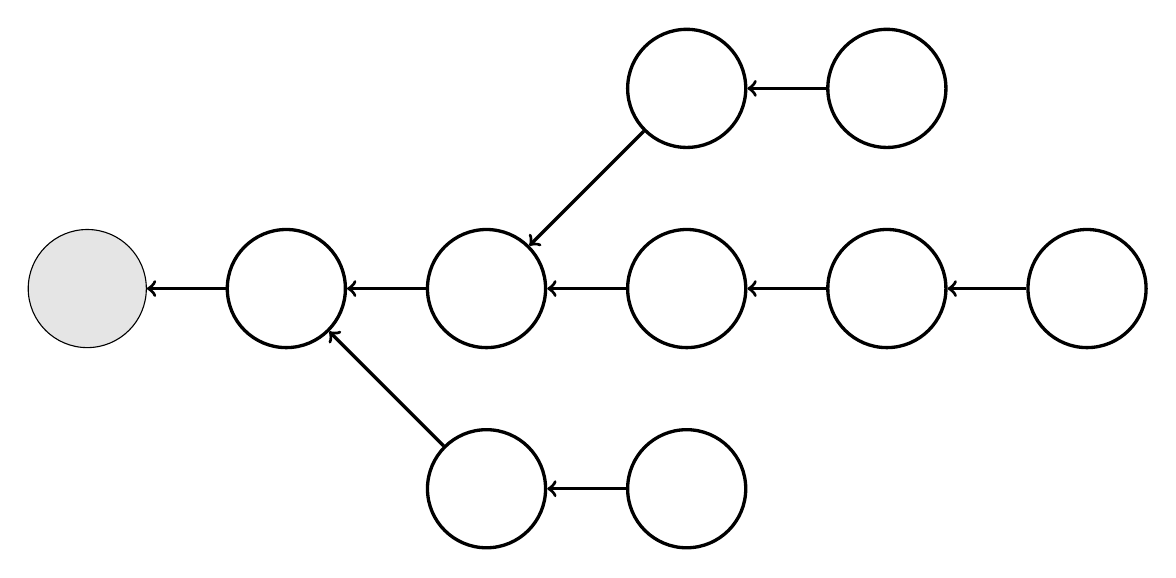
\begin{tikzpicture}[
				block/.style={circle, draw=black!100, very thick, minimum size=1.5cm},
				invis/.style={circle, draw=black!100, fill=black!10, minimum size=1.5cm}
			]
			\node[invis] (genesisblock) {};
			\node[block] (block1) [right=of genesisblock] {};
			\node[block] (block2) [right=of block1] {};
			\node[block] (block3) [right=of block2] {};
			\node[block] (block4) [right=of block3] {};
			\node[block] (block5) [right=of block4] {};
			\node[block] (sub1) [below=of block2] {};
			\node[block] (sub2) [below=of block3] {};
			\node[block] (sub3) [above=of block3] {};
			\node[block] (sub4) [above=of block4] {};
			\begin{scope}[very thick, -stealth]
			\draw[<-] (genesisblock.east) -- (block1.west);
			\draw[<-] (block1.east) -- (block2.west);
			\draw[<-] (block2.east) -- (block3.west);
			\draw[<-] (block3.east) -- (block4.west);
			\draw[<-] (block4.east) -- (block5.west);
			\draw[<-] (sub3.east) -- (sub4.west);
			\draw[<-] (block1.south east) -- (sub1.north west);
			\draw[<-] (sub1.east) -- (sub2.west);
			\draw[<-] (block2.north east) -- (sub3.south west); 
			\end{scope}
			\end{tikzpicture}
			\end{center}
		\caption{A typical blockchain structure}
		\label{fig:mainblockchain}
	\end{figure}
	The blockchain, as a cryptographically secure chain of blocks, was first conceptualised by Stuart Haber and W. Scott Stornetta in 1990 \cite{HaberStornetta}.
	However, until the creation of Git \cite{Git} in 2005, the blockchain was still a relatively niche concept.
	The invention of Bitcoin in 2008 is seen by many as the most pivotal moment in the history of blockchain technologies.
	Bitcoin uses the Proof of Work consensus algorithm to create a decentralised, trust-less, peer to peer network which is used to make transactions between virtual wallets.

	\section{Blockchain Today}
	At the time of writing, cryptocurrencies are generating both a huge amount of excitement and cynicism in popular media. 
	Aside from Bitcoin, cryptocurrencies like Ethereum \cite{Ethereum} have introduced the concept of Smart Contracts which allow the execution of code on the blockchain.\\
	
	Whilst it is possible to think of applications for blockchain technology in almost every sector, the development of applications outside the scope of crytocurrencies has been limited. 
	If one considers the example of OCaml, there are currently no libraries which allow a user to easily get started with building blockchain applications. \\

	\section{Work Completed}
	I have created Logan which is a library that allows developers to create blockchain applications with the ease of importing a library.
	Logan was designed to exist outside the realm of cryptocurrencies and therefore assumes that all participating nodes are trustworthy.
	Consensus is achieved by using a simple leader-based mechanism where the leader node will periodically pull updates from all participating nodes and add them to a central blockchain.
	This can then be viewed by all participating nodes, with the guarantee of strict consistency.
	Setting up a network is as easy as specifying the location of the leader on all the participating nodes, and specifying the location of all participating nodes on the leader.\\
	
	I have evaluated the project by... FILL IN EVALUATION DETAILS

	\chapter{Preparation}
	Before starting work on the project code, I completed a lot of preparation in order to aid the development process.
	I spent some time learning to use OCaml and familiarising myself with its features.
	This was important because it allowed me to write idiomatic code which was not only powerful, but could also provide an intuitive API for other developers to use.
	I also spent some time investigating a few key libraries, such as Irmin and Lwt.
	Understanding these libraries, the data structures they provide, and the technologies they present, allowed me to focus on the technological challenges in the project and not waste time reinventing the wheel. 
	Setting up a good development environment allowed me to run automated builds and, therefore, catch any errors in the code early.
	This was particularly useful during the evaluation as it involved installing the project on many remote machines.
	Being able to catch issues like dependency resolution or out of date build commands made the evaluation process much easier.
	Lastly, I spent some time developing a requirements analysis for the final product. 
	This analysis helped drive the design and development of the blockchain library whilst not restricting the work that I was able to complete.

	\section{Starting Point}
	The project built upon functionality provided by Irmin [1] which is a distributed database system.  Irmin is fast, durable and has all the necessary capabilities required to build a blockchain.
	The project also made use of Ezirmin \cite{Ezirmin} which provides a simplified API to Irmin, and defines a log data structure which was used to build the blockchain and mempool structures for this project.

	\section{Using OCaml}
	At the start of the project, I had never used OCaml for any project of significance. 
	Whilst the first year Foundations of Computer Science course had given me some background into functional programming, there were still many key OCaml features which I had to learn.
	In the first few weeks of my project, I spent time studying the book Real World OCaml \cite{RealWorldOCaml} which proved a great introduction to many of OCaml's features.  

	\subsubsection*{Pattern Matching}
	OCaml provides a very powerful syntax for matching patterns which allow you to write functions as shown by Listing \ref{lst:pattern_match}.
	\begin{lstlisting}[caption={OCaml Pattern Matching}\label{lst:pattern_match}]
let pattern_matcher_1 input = match input with
  | Card("spades", 1) -> Printf.printf "It's the ace of spades!"
  | _ -> Printf.printf "Unlucky"
let pattern_matcher_2 = function
  | Card(suit, 1) -> Printf.printf "It's the ace of %s!" suit
  | _ -> Printf.printf "Unlucky"
	\end{lstlisting}
	Listing \ref{lst:pattern_match} shows a function that will print a special string if it is passed the Ace of Spades. 
	Here, the pattern matching checks the that the tuple associated with the data type contains the string \texttt{spades} and the number 1.
	The second example assigns the variable \texttt{pattern\_matcher\_2} to an anonymous \texttt{function} which matches the first argument of the tuple to the variable \texttt{suit}.
	\subsubsection*{Options}
	An \texttt{Option} is a built in data type that provides a powerful way of using OCaml's pattern matching.
	By using the \texttt{Some(\ldots)} and \texttt{None} constructors, one can create something of the type \texttt{'a option}. 
	This is comparable to the \texttt{null} type in languages such as Java, however as it is part of the type system, it forces the programmer to handle any cases where \texttt{null} could be returned.

	\subsubsection*{Error Handling}
	OCaml provides multiple different ways of dealing with errors and exceptions. 
	A simple way of signifying an error in your return type, is to return an \texttt{option} which will be \texttt{None} if there is an error. 
	Whilst this can be inflexible for larger solutions, it also provides a quick and simple way of signifying that something has gone wrong.\\

	Another way of dealing with options in return types is to use the \texttt{bind} function:
	\begin{lstlisting}
val bind: 'a option -> ('a -> 'b option) -> 'b option = <fun>
	\end{lstlisting} 
	As the type signature demonstrates, \texttt{bind} takes an \texttt{option} and applies a function to its contents if it exists, or returns \texttt{None} otherwise.\\
	
	OCaml provides a built in type \texttt{Result.t} which is an extension of optional return types, where the programmer is able to define arbitrary data to accompany the error type. 
	The following demonstrates a successful return type of \texttt{int} (with an unspecified \texttt{Error} type), and a \texttt{string} error type (with an unspecified \texttt{Ok} type).
	\begin{lstlisting}
# Ok 3;;
- : ('a, int) result = Ok 3
# Error "Something went wrong";;
- : (string, 'a) result = Error "Something went wrong";;
	\end{lstlisting} 

	\subsubsection*{Polymorphic Variants}
	OCaml allows the programmer to define variant types such as the \texttt{Card} type that was defined earlier. This makes it very easy to make use of pattern matching with custom defined types.\\
	
	OCaml also introduces the notion of polymorphic variants which are more flexible and do not require an explicit type declaration.
	\begin{lstlisting}[caption={Polymorphic Variants}\label{lst:poly}]
# let card = `Card ("spades", 1);;
- : val card : [> `Card of string * int ] = `Card ("spades", 1)
	\end{lstlisting}
	Listing \ref{lst:poly} shows how a back-tick can be used to define a polymorphic type, and OCaml has automatically inferred a type. 
	The $>$ symbol acts as a lower limit on the tags that the variant \texttt{card} can take, i.e. it can have the tag \texttt{Card} or any other unspecified tag.
	When dealing with variant types as \textit{parameters}, the $<$ symbol often appears in the type signature to show that the parameter can belong to only a subset of given set of tags. T
	The absence of both of these symbols indicates that a variant can take any value from the given set of tags, rather than a superset or subset. 

	\subsubsection*{Modules and Functors}
	Modules provide a way of grouping together related code in OCaml.
	They can be thought of as similar to traditional namespaces, although there a few key differences.
	OCaml also lets you define module type signatures which modules have to conform to.
	\begin{lstlisting}[caption={OCaml Modules and Functors}\label{lst:modfun}]
module type Math = sig
  type t
  val add: t -> t -> t
  val subtract: t -> t -> t
end

module IntegerMath : Math with type t = int = struct 
  type t = int
  let add int1 int2 = int1 + int2
  let subtract int1 int2 = int1 - int2
end
	\end{lstlisting}
	Listing \ref{lst:modfun} is a simple example that defines a module signature \texttt{Math} for adding and subtracting a custom type.
	The module \texttt{IntegerMath} is a module which adheres to this signature. 
	The syntax \texttt{with type t = int} serves the purpose of letting the compiler know that the type t is externally visible.
	Whilst this example uses the trivial example of integer maths, it is easy to imagine this extending to, for example, matrices or sets where these functions are not part of the language.\\

	Modules are really useful for allowing the effective division of code into isolated units, but on their own, they are slightly inflexible. 
	Maybe a developer would want to abstract some lower level details of code used by a module.
	In this case, she would have to create a whole new module for each possible implementation of this abstraction.
	An example of this could be a datastore that uses either an in-memory or on-disc format for storing data.
	Functors allow modules to be created from other modules.
	\begin{lstlisting}[caption={Ezirmin Log Module}\label{lst:logmod}]
module Log(AO : Irmin.AO_MAKER)(V: Tc.S0) = struct
  ...
end
	\end{lstlisting}
	Listing \ref{lst:logmod} is an example from the Ezirmin codebase and shows how to define a functor.
	The parameter \texttt{AO} is a module used for creating append only stores, and the parameter module \texttt{V} defines a data type.
	The result of this is a functor, \texttt{Log}, which can be used to create a Log module with either an in-memory or on-disc backend.
	\subsubsection*{Development Environment}
	When developing a large scale system with OCaml, there are a couple of build systems available to use. 
	`jbuilder' \cite{jbuilder} is one of these systems which is becoming increasingly popular and is used daily by hundreds of developers.
	jbuilder allows the developer to specify arbitrary directory structures containing executables, libraries and more.
	I set up my project to compile Logan, which includes the interface for running both Leader and Participant nodes. 
	I also defined multiple executables for running both the Leader and Participants in example and test cases. 
	I used GNU Make \cite{GNUMake} to invoke jbuilder which allowed me to easily build and run any executables from the root of the directory.\\
	
	In order to ensure that the project would always build, I set up a continuous integration workflow using Travis-CI. 
	This ensured that whenever I pushed any updates to my GitHub repository, Travis would attempt to build the system and would notify me whenever there were any errors during the build.
	This was particularly useful during the Evaluation stage when I was installing my project on multiple remote machines for testing.
	Over the development period, Travis flagged issues such as dependency resolution failures or out of date build scripts and I was able to fix these at the point when they first occurred, rather than weeks later when they would have caused many issues during remote installation.

	\subsubsection*{Lwt}
	A library which I spent some time familiarising myself with was Lwt \cite{Lwt}. 
	Lwt provides a way of interacting with threads in OCaml, although in Lwt they are known as `Promises'.
	\begin{lstlisting}[caption={Lwt Promises}\label{lst:lwt}]
val Lwt.return : 'a -> 'a Lwt.t 
val Lwt_main.run : 'a Lwt.t -> 'a
val Lwt.bind : 'a Lwt.t -> ('a -> 'b Lwt.t) -> 'b Lwt.t
	\end{lstlisting}
	Listing \ref{lst:lwt} shows the basic functions for creating, running and combining threads.
	The above type \texttt{'a Lwt.t} refers to a thread which will eventually terminate with a value of type \texttt{'a}, and follows the well established Monad design pattern.
	\texttt{Lwt.return} is a function that takes a value and will create a promise that immediately returns with this value.
	This is useful when inserting static or precomputed variables into Lwt pipelines.
	\texttt{Lwt\_main.run} is the dual of \texttt{Lst.return} and will run a Lwt promise until completion and then return its value.
	This is useful when retrieving values from an Lwt pipeline.
	Finally, \texttt{Lwt.bind} (or the infix notation \texttt{>>=}) will pass the result of a Lwt promise to a function returning another Lwt promise.
	This is useful for chaining together Lwt promises in a pipeline.

	\section{Requirements Analysis} \label{Requirements Analysis}
	During the preparation stage of my project, I spent some time analysing the requirements that would be suitable for Logan. 
	This proved a good way of guiding the progress of the project and making sure that I solved all the problems that I set out to. 
	Here, I will set out the criteria that I decided upon before starting development on the project.
	\subsection{Data Structure}
	One of the most important requirements for Logan, is that it should be able to add items to and view items in a blockchain. 
	The data in the blockchain will be referred to as either \textit{blocks} or \textit{transactions}. 
	From a participating node, it should be possible to add a transaction, of arbitrary type. 
	It should also be possible to view an ordered list of all transactions which currently exist in the blockchain.
	The latency of adding transactions should not increase as the size of the blockchain increases because it is important the library will cope well with systems running for an indefinite period of time.\\

	\begin{minipage}{\linewidth}
	\begin{lstlisting}[caption={Blockchain Specification}\label{lst:blockspec}]
module type I_LogStringCoder = sig
  type t
  val encode_string: t -> string
  val decode_string: string -> t option
end

module type I_Validator = sig 
  type t 
  val init: t list -> unit Lwt.t 
  val filter: t list -> t list Lwt.t
end

module type I_Config = sig
  type t
  module LogCoder: I_LogStringCoder with type t = t
  module Validator: I_Validator with type t = t
  val remotes: string list
end

module type I_Blockchain = sig
  type t
  val add_transaction_to_blockchain: t -> [> `Error | `Ok] Lwt.t
  val get_all_transactions: unit -> [> `Error | `Ok of t list] Lwt.t
  val get_transactions: int -> [> `Error | `Ok of t list] Lwt.t
end

module Make(Config: I_Config): I_Blockchain with type t = Config.t = struct 
  ...
end
	\end{lstlisting}
	\end{minipage}\\
	\\
	Listing \ref{lst:blockspec} is the initial technical specification that I used to define Logan, and the functions complete the following operations:
	\begin{itemize}
		\item \texttt{I\_LogStringCoder} is a module that allows the user to specify arbitrary types to be stored on the blockchain, so long as they can be encoded to (and decoded from) a string.
		\item \texttt{I\_Config} contains information which is required to run the blockchain, including \texttt{remotes} which is a list of other participating nodes.
		\item \texttt{I\_Validator} is an interface which is defined by the library user. 
			Validation is performed by initialising a \texttt{Validator} module with the transactions already committed to the blockchain.
			From then on, \texttt{Validator.filter} will take a list of requested transactions and will return a subset of them which are the valid transactions.
			The \texttt{Validator} can then assume that these transactions have been committed for future calls to \texttt{filter}.
		\item \texttt{Make} is a functor which accepts a configuration module and will return a blockchain module.
		\item \texttt{add\_transaction\_to\_blockchain} adds a user defined type to the blockchain and then returns a polymorphic variant type containing information about whether the operation was successful. 
			This will return an error in the case that the transaction is not validated.
	\end{itemize} 
	This specification differs slightly from the final specification for Logan because it does not take into account the difference between Leader and Participant nodes.
	The specification was deliberately designed without focus on consensus so that the focus was on the external functionality rather than the internal implementation. 
	The final interface, while different, provides exactly this functionality.

	\subsection{Consensus}
	Ensuring that Logan maintains consensus was a very crucial part of this project. 
	The actual design and development of the consensus algorithm was completed throughout the duration of the project and involved a lot of research into other consensus mechanisms.
	However, during the requirements analysis phase of the project I set out some goals for the final implementation.
	These goals were laid out in order to help drive the design and development of the consensus mechanism. 
	I decided on the following requirements:
	\begin{itemize}
		\item The consensus mechanism must guarantee strict consistency. Although strict consistency could add large overhead costs, it is necessary for some applications and so is an important part of the final project.
		\item The consensus mechanism must be scalable. Within the scope of this project, it should be possible for the blockchain to be shared by 3 or more nodes in a network. This should not hinder the performance of the system, and it should still be able to handle multiple successful transactions per second.
	\end{itemize}

	\chapter{Implementation} \label{Implementation}
	Over the course of this project, I have successfully built Logan, a blockchain library which can perform custom transaction validation.
	Logan uses a Leader based consensus protocol inspired by Raft also uses the concept of a `transaction waiting room', or \textit{mempool}, which is used by Bitcoin.
	Section \ref{sec:sysarch} gives a general overview of Logan's system architecture.
	Section \ref{sec:datastructure} describes the blockchain data structure that I have used, and justifies why it can be considered a blockchain.
	I will also describe two bugs that I encountered in these codebases and the fixes that I implemented for each.
	Finally, Section \ref{sec:consensus} gives a description of the research I completed when designing Logan's consensus mechanism. 
	I will first present a naive approach to consensus and explain why this is flawed and will cause transactions to be committed out of order.
	I will then present an improved mechanism, which Logan uses, that guarantees that no transactions in participant mempools are missed.

	\section{System Architecture}\label{sec:sysarch}
	Logan's goal is to allow multiple nodes in a distributed system to share a blockchain data structure.
	Nodes in this system should be able to add transactions to the blockchain and read the entire history of previous transactions.
	Logan aims to achieve this goal by using a Leader-based approach where a \textit{Leader} node can accept transactions from \textit{Participant} or \textit{Worker} nodes and commit them to the blockchain for everyone to see.
	Participants view the blockchain by retrieving the latest copy over an SSH connection with the Leader.
	Participants request for transactions to be committed by writing to their local mempool. 
	The Leader periodically polls the Participant mempools, again over an SSH connection, to find new transactions to add to the blockchain.
	When a poll finds new transactions, it will use the Validation module to filter for all the valid transactions which are then added to the blockchain.
	It is also possible for a Participant node to exist on the same physical machine as the Leader, in which case the Leader sources updates directly from the mempool, rather than over an SSH connection. 
	Figure \ref{fig:sysarch} shows how the architecture for this system is organised.\\	

	\begin{figure}
		\centering
		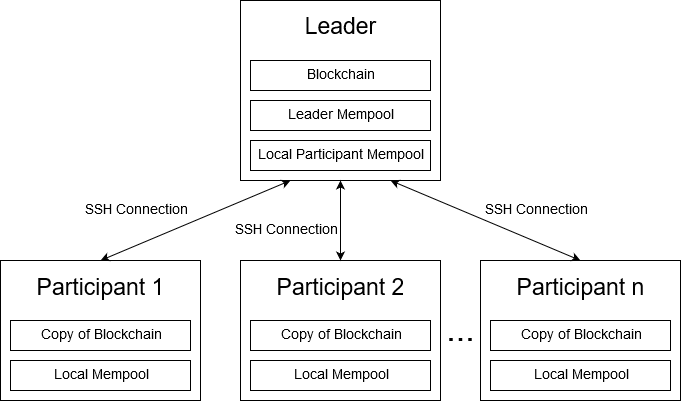
\includegraphics[width=16cm]{figs/System_Architecture.png}
		\caption{Logan system architecture overview}
		\label{fig:sysarch}
	\end{figure}

	\section{The Blockchain Data Structure}\label{sec:datastructure}
	Irmin is a library for OCaml providing datastore functionality using a Git backend.
	Ezirmin is a wrapper around Irmin that provides a simple log data structure which I have used as a blockchain.
	In order to justify that this data structure can be considered a blockchain, I took some time to investigate its semantic properties. 
	Whilst there is no universally agreed-upon definition of a blockchain, I have used the following criteria to define the blockchain:
	\begin{enumerate}
		\item Data is stored in `blocks'.
		\item Blocks are ordered in a tree structure where each block contains the hash its parent block.
	\end{enumerate}
	This definition deliberately makes no mention of consensus, and exists purely to justify the validity of the blockchain data structure.
	\subsection{Irmin}
	Irmin is a library for OCaml which provides Git-like, distributed, branchable storage \cite{Irmin}. 
	Irmin exposes three main structures as shown in Figure \ref{fig:IrminBlockStore}: The Block Store, the Tag Store and the Irmin Store.
	\begin{figure}
		\begin{center}
		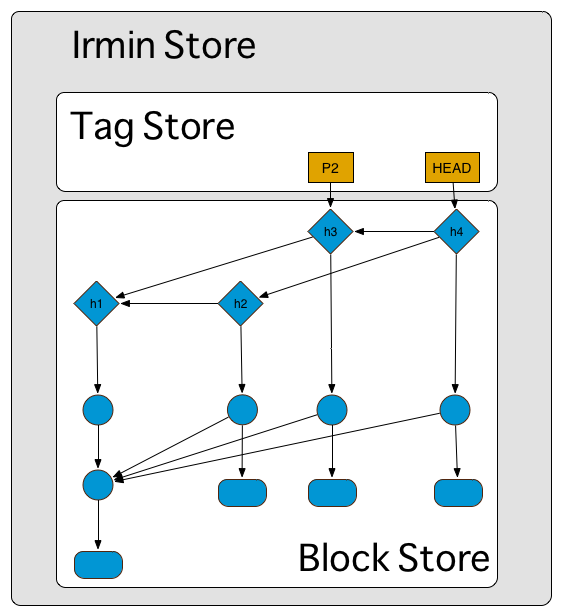
\includegraphics[width=13cm]{figs/irmin-stores.png}
		\caption{Architecture of an Irmin Store}
		\label{fig:IrminBlockStore}
		\end{center}
	\end{figure}
	For the reader familiar with Git, these can intuitively be thought of as objects/commits, branches and repositories respectively.
	\subsubsection*{The Block Store}
	The Irmin Block Store is a heap of immutable blocks. 
	Rather than being addressed by a physical address, these blocks are addressed by the hash of their content.
	Because the Block Store is content-addressable, once blocks are added, their content can never be updated.
	Instead, updates to Irmin data structures will add new blocks which try to utilise as much shared history with the existing data in the store, in order to minimise storage space.
	\subsubsection*{The Tag Store}
	Any immutability in Irmin data structures derive from \textit{tags}.
	Tags provide a way of indexing into any block in the Block Store.
	This concept is similar to that of branches or references in Git, which provide a way of indexing into a particular commit in the Git history.
	Because blocks are immutable, any changes to an Irmin data structure can only be visible if a tag is updated. 
	In particular, I will refer to the HEAD tag or pointer, which will index into the latest recognised log item.
	When Irmin merges data structures, it creates new blocks and updates the relevant tags to point to these, however, the old blocks remain in the block store.
	\subsubsection*{Irmin Stores}
	An Irmin Store is simply the combination of a Block Store and a Tag Store.
	Considering the criteria set out earlier for a data structure to be considered a blockchain, Irmin Stores satisfy the first criteria, i.e. that data is stored in Blocks.
	Indeed, they also come close to satisfying the second criteria, as all blocks are indexed by the hash of their content. 
	However, this is not quite enough, as blocks are not required to contain hashes of parents in a chain.
	In order to satisfy these criteria, I looked to Ezirmin which provides a log data structure.

	\subsection{Ezirmin}
	Ezirmin is a library that provides a simplified interface to the Irmin library. 
	It is designed to provide a interface to Irmin without functors, but with some useful defaults. 
	Importantly, it has a built in log data structure which uses Irmin's append-only store, saved on disk in the Git format.

	\begin{lstlisting}[caption={Ezirmin Log}\label{lst:ezirminlog}]
module type FS_Log = sig
  type elt 
  type cursor 
  val append : ?message:string -> branch -> path:string list -> elt -> unit Lwt.t
  val get_cursor : branch -> path:string list -> cursor option Lwt.t
  val read : cursor -> num_items:int -> (elt list * cursor option) Lwt.t
  val read_all : branch -> path:string list -> elt list Lwt.t
  ...
end
	\end{lstlisting}

	Listing \ref{lst:ezirminlog} gives some of the interface for an Ezirmin log which uses a file system backend.
	The log allows for items to be appended to and read from a log, and the concept of cursors here maps directly to the concept of Irmin tags.
	In particular, the function \texttt{read} will read from the item indexed by a cursor, and will return a new cursor for the next unread log item, alongside the result of the read.

	\subsubsection*{Ezirmin Log as a Blockchain}
	Logan uses an Ezirmin Log as an implementation of a blockchain, but to verify that this is a valid data structure to use, I investigated the implementation of Ezirmin Logs.
	Ezirmin Logs use Irmin blocks to store log entries, and therefore satisfy the first criteria for being considered a blockchain. 
	To verify that they also satisfy the second criteria, i.e. that blocks are ordered and contain the hash of their parent, I looked at the implementation of log items.

	\begin{lstlisting}[caption={Ezirmin Log Item}\label{lst:a_label}]
type log_item =
{ time    : Time.t;
  message : V.t;
  prev    : K.t option}
	\end{lstlisting}

	Listing \ref{lst:a_label} is taken from the Ezirmin Log implementation and shows how each log item has a \texttt{prev} value which is a key pointing to its parent log item. 
	This imposes an ordering of log items, and means that any changes to previous log items will not be observed, as they will simply create a new block with a new address. 
	Merging Ezirmin Logs causes new \texttt{Merge} blocks (as opposed to \texttt{Value} blocks) to be created that collate multiple log entries from divergent log histories.
	These entries are ordered by their timestamps and this means that after a merge, items may appear to have been inserted into the log history.
	This is not desirable behaviour for a blockchain, so I have ensured that the blockchain data structure maintained by Logan is never merged with other structures, only appended to. 
	Consequently, each blockchain transaction will exist in its own \texttt{Value} block and will never removed or reordered in the blockchain.
	Therefore it can be concluded that an Ezirmin Log satisfies both of my conditions to be considered a blockchain.

	\subsubsection*{Merging Ezirmin Logs}
	Aside from using an Ezirmin Log as the blockchain data structure for this project, I also use a \textit{mempool} log to retrieve updates/transactions from remote mempools. 
	This retrieval process uses the \texttt{Ezirmin.Repo.Sync} module to merge new log items into the Leader's mempool.
	Under the hood, this module uses the git protocol to pull updates over an SSH connection.
	In this section I will investigate the semantics of Ezirmin merges as they are critical to understanding how Logan achieves consensus.\\
	
	Irmin allows for the developer to specify custom merge strategies. 
	Whenever a Irmin Store merges changes from a remote Store, Irmin will do one of two things:
	\begin{enumerate}
		\item If the newly discovered blocks do not have a divergent history to the current store, they will simply be added to the Block Store. 
			In other words, if only new blocks have been added in the remote store, these will be added to the local store. 
		\item If the remote and local stores have divergent histories, then a custom three way merge is made using the heads of each store and their latest common ancestor.
			This merge is defined by the developer.
	\end{enumerate}
	Figure \ref{fig:ezirminmerges} shows how a local Ezirmin Log performs a merge from a remote log with a diverging history.
	Before the merge, the local store has a \texttt{Value} block, \texttt{V1}, but the remote store has a different \texttt{Value} block, \texttt{V2}.
	After the local store has merged changes from the remote store, a new \texttt{Merge} block, \texttt{M1,2}, has been created which contains both histories as defined by the custom merge function. 
	Blocks \texttt{V1} and \texttt{V2} still exist in the block store, but the HEAD tag has been updated to point to \texttt{M1,2}. \\

	\begin{figure}
		\centering
		\begin{subfigure}[t]{0.40\textwidth}
			\centering
			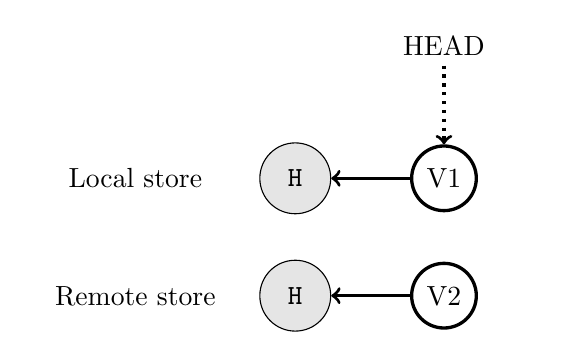
\begin{tikzpicture}[
				block/.style={circle, draw=black!100, very thick, minimum size=7mm},
				invis/.style={circle, draw=black!100, fill=black!10, minimum size=9mm},
				label/.style={rectangle, text width=2.5cm, align=center}
			]
			\node[label] (local) {Local store};
			\node[label] (remote) [below=of local] {Remote store};
			\node[invis] (gentop) [right=2mm of local]{\texttt{H}};
			\node[block] (history1) [right=of gentop] {V1};
			\node[label] (head) [above=of history1] {HEAD};
			\node[invis] (genbottom) [right=2mm of remote] {\texttt{H}};
			\node[block] (history2) [right=of genbottom] {V2};
			\begin{scope}[very thick, -stealth]
			\draw[->, dotted] (head.south) -- (history1.north);
			\draw[<-] (gentop.east) -- (history1.west);
			\draw[<-] (genbottom.east) -- (history2.west);
			\end{scope}
			\end{tikzpicture}
		\caption{Two Ezirmin logs diverging from a shared history, \texttt{H}.}
		\end{subfigure}
		\begin{subfigure}[t]{0.5\textwidth}
			\centering
			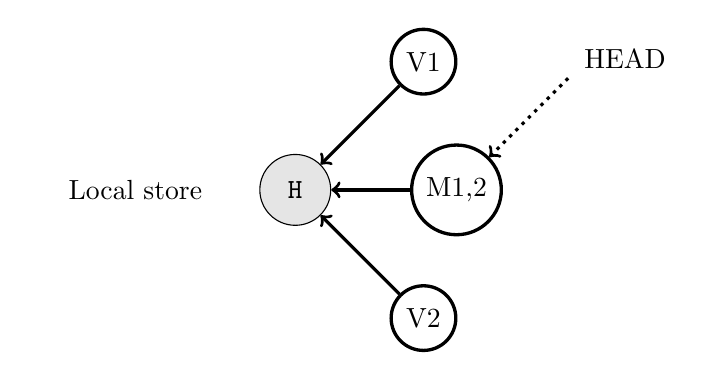
\begin{tikzpicture}[
				block/.style={circle, draw=black!100, very thick, minimum size=7mm},
				invis/.style={circle, draw=black!100, fill=black!10, minimum size=9mm},
				label/.style={rectangle, text width=2.5cm, align=center},
				labelhead/.style={rectangle, text width=1.2cm, align=center}
			]
			\node[label] (local) {Local store};
			\node[invis] (gentop)[right=2mm of local] {\texttt{H}};
			\node[block] (history1) [above right=of gentop] {V1};
			\node[block] (history2) [below right=of gentop] {V2};
			\node[block] (merge) [right=of gentop] {M1,2};
			\node[labelhead] (head) [above right=of merge] {HEAD};
			\begin{scope}[very thick, -stealth]
			\draw[->, dotted] (head.south west) -- (merge.north east);
			\draw[<-] (gentop.north east) -- (history1.south west);
			\draw[<-] (gentop.south east) -- (history2.north west);
			\draw[<-] (gentop.east) -- (merge.west);
			\end{scope}
			\end{tikzpicture}
			\caption{After the local log has merged changes from the remote log, the HEAD tag now point to a merge item, \texttt{M1,2}, which is generated by the custom merge function.}
		\end{subfigure}
		\caption{Merging Ezirmin Logs}	
		\label{fig:ezirminmerges}
	\end{figure}

	\subsubsection*{Ezirmin Bugs}
	Whilst Ezirmin provides a set of very desirable semantic properties, it is not a widely used library. 
	Consequently, during the course of the project, I encountered bugs in the Ezirmin codebase which I had to debug and fix.
	In this section I shall outline the two bugs that I encountered the changes I made to the Ezirmin codebase to fix them.\\
	
	The first bug occurs when updates are merged into a log over a network.\footnote{The issue on GitHub can be found at \href{https://github.com/kayceesrk/ezirmin/pull/7}{https://github.com/kayceesrk/ezirmin/pull/7}}
	Irmin uses Git as a backend and in order to merge updates over a network, the \texttt{git pull} command is used.
	In Git, objects are stored as blobs on the leaves of a tree and \texttt{git pull} works by retrieving all blobs at the leaf nodes of the tree for a given branch.
	However in Ezirmin, blobs can contain pointers to other blobs, and \texttt{git pull} will not know to retrieve these blob too.
	This will cause an error when Ezirmin tries to read these objects which do not actually exist locally. 
	The solution that I implemented to this problem is to use an internal branch which uses an Irmin Store to explicitly track every blob in the log.
	Items are added to this Irmin Store on the internal branch every time they are added to the log.
	This operation inserts these blobs into the git tree such that if \texttt{git pull} is performed on the internal branch, all the blocks required by the master branch will be retrieved.\\

	The second bug that I encountered derived from the merge behaviour of Ezirmin logs when there are more than two remote machines merging updates from each others' log.\footnote{The issue on GitHub can be found at \href{https://github.com/kayceesrk/ezirmin/pull/8}{https://github.com/kayceesrk/ezirmin/pull/8}}
	The issue is that when a \texttt{Merge} block is created, it may contain log items which, on other machines, are stored as \texttt{Value} blocks or as different \texttt{Merge} blocks.
	The result is that Irmin sees these blocks as different, and Ezirmin does not perform any checks to detect or remove duplicate log items occuring in different contexts.
	This behaviour resulted from complex sequences of merge operations and so was difficult to reproduce, but in the worst case caused the size of the blockchain to grow exponentially with the number of merge operations performed.
	In one case, a log with 40 unique log items grew to be greater than 120,000 log items in size due to duplicates.
	I implemented a fix by removing duplicate log items when a merge operation takes place. 
	Duplicates are found by comparing the log item timestamps, and whilst this does not guarantee their individuality, the timestamps have such significant precision to make this highly unlikely.

	\section{Consensus Algorithms}\label{sec:consensus}
	Building consensus was by far the most important part of work completed for this project. 
	In order to guide the design of the consensus mechanism, I completed an extensive amount of research on existing algorithms
	This section will briefly summarise this research and my conclusions about their suitability for Logan. 
	The resulting design for consensus is a leader based approach, where Participants can commit transactions to a mempool.
	The Leader polls these mempools for updates, which are validated and then committed to the blockchain.
	This blockchain can be read by all Participants, and provides a definitive source of ordered, committed transactions.

	\subsection{Building Consensus}
	\subsubsection*{Proof of Work}
	%TODO: Use a diagram,
	Proof of Work (PoW) is a deceptively simple consensus mechanism, used by most cryptocurrencies to avoid the double spending problem.
	Transactions are contained within blocks which can be broadcast out to the network of participating nodes. 
	Whenever a block is received by a participating node, the node checks that the block contains a proof of computational work done. 
	This proof usually takes the form of a random sequence of data (this is known as a nonce) appended to the end of the block, causing the block's hash to be prefixed with a set number of 0s.
	This acts as a proof of computational work, because the data appended to the end of a block can only be found by a brute force method called mining, but can also be verified easily by simply computing the block's hash.\\
	
	Why is this useful? 
	Well, this makes a guarantee on the validity of the blockchain based on the simple assumption that more that 50\% of the workforce is genuine.
	That is, ifm we assume that the longest chain of blocks is the correct one, then in order to create a sequence of biased transactions, we would have to create a chain longer than the correct one. 
	This would require an equal number of `Proof of Work's, which, due to the random nature of block mining, would require more than 50\% of the workforce.
	Whilst it may be possible to maintain an equally sized chain with less that 50\% of the workforce for a short period of time, the chances of this decrease rapidly as time passes.
	All in all this means that the longer a block has been in the chain, the more likely it is that the block is valid.\\

	Whilst this forms a very effective mechanism for achieving consensus, there are also some considerable downsides to using a PoW approach to consensus. 
	Firstly, there is a huge amount of computational work wasted in the process of mining. 
	The effect of this is energy consumption \cite{BitcoinEnergy} and wastage to a level which can cause serious environmental harm.
	PoW also does not generalise well outside of the scope of cryptocurrencies.
	It assumes no trust in any participants which may not be a suitable model for an application. 
	Additionally, it also assumes that miners can be rewarded, usually with cryptocurrency, but this incentive is ad hoc and may not exist in other applications.
	
	\subsubsection*{Mempools}
	Mempools are an important part of the design of Bitcoin, and whilst they are not inherently linked to the Proof of Work consensus algorithm, they are worth investigating. 
	When a Bitcoin transaction is made, it is first written into what is known as a Mempool. 
	This transaction can then be seen by participating miners, who can then choose to put this in the next block that they mine. 
	This is significant, as it provides a `waiting room' for any transactions that have not yet been validated.  

	\subsubsection*{Proof of Stake}
	The Proof of Stake (PoS) algorithm is used by some cryptocurrencies and works by randomly allowing participants to create (or `forge') a single block.
	However, the probability that a participant is chosen to `forge' a block, is weighted by its stake, such that participants with higher stakes in the blockchain are more likely to be chosen to forge a block.\\

	So, why is PoS desirable? 
	By far the most convincing reason for using PoS over PoW, is that there is no need to waste lots of energy in the process of mining. 
	This hugely reduces the environmental impacts of scaling a PoS network.
	Using PoS also allows trust to be distributed according to an arbitrary heuristic which can be desirable property in some applications.\\

	One of the flaws of PoS is that it does not have such a strong deterrent against attacks.
	With PoW, attacks require huge amounts of computational power and it is likely that to create an attack, you would have to spend more on hardware than you would gain. 
	PoS does not have this same built in mechanism, and so there have been many suggested schemes for increasing the safety of PoS networks.
	For example, it is possible that participants should need to pay some form of deposit before forging blocks, which can be slashed if they break any rules. 
	PoS also suffers from the same problem as PoW in that it does not generalise well. 
	It is another example of a consensus mechanism designed for networks with a strong notion of Stake and with minimal trust in any individual participant.

	\subsubsection*{Paxos}
	Paxos is a family of consensus protocols which can be used to guarantee consistency in distributed systems. 
	It was first proposed in a paper by Leslie Lamport in 1998 \cite{Paxos}, although the paper was first submitted in 1990.
	Named after a fictitious civilisation living on the island of Paxos, the algorithm puts forward a way for any number of nodes to propose and agree on a value.
	Participating nodes belong to various roles, one of which is known as a `Proposer' or Leader.\\

	The main part of the algorithm is split into two sections, propose and accept.
	In the first stage, a Proposer decides that it wants to propose a value and then broadcasts out a `Prepare' message to a quorum of `Acceptors'.
	Acceptors will then decide if they want to make a `Promise' which is a commitment to accepting that proposal in the future. 
	If a quorum of promises is received by the Proposer, then it will assign a value to its proposal and will again send an `Accept Request' out to a quorum of Acceptors.
	Finally, if enough `Accept' messages are received then the Proposer can be certain that the value has been agreed upon by consensus.\\

	This algorithm has been proved to be consistent but it also has a lot of complexity and a lot of different variants. 
	The combination of different roles and states makes it easy to implement incorrectly.
	It is also important to consider that Paxos describes a `family' of algorithms, with some parts left deliberately unspecified, and choosing how to implement these is not a trivial decision.
	The final issue with Paxos is that it cannot guarantee progress.
	Whilst it enforces conditions which make it unlikely that progress will not be made, it is still theoretically possible for the mechanism to stall indefinitely.

	\subsubsection*{Raft}
	Raft \cite{Raft} is an algorithm that was designed to be equivalent and as efficient as Paxos, however, it also places a much greater emphasis on comprehensibility.
	It uses the notion of a \textit{strong leader}, which is an elected server that has total control over which log entries are accepted.
	There are two other types of server, a \textit{follower} and a \textit{candidate}. 
	Followers are completely passive, and only respond to requests from leaders and candidates. 
	A candidate is a server that has put itself forward for election.\\

	So how does the algorithm operate? 
	Time in Raft is split into \textit{terms} which are labelled by a monotonically increasing integer. 
	Each term effectively signals a time period where a particular server is the leader. 
	A term starts with a leadership election when a follower transitions into the candidate state, increments its term number and requests votes from other servers. 
	It will wait for a majority of votes and then elect itself the leader, unless it times out or receives a message from another leader with a greater term number. 
	Typically, these leader election processes are triggered when a follower does not receive a heartbeat message from the leader for longer than a given time.
	In the pathological case, the vote can be split between leaders, triggering a new election which is also split and so on.
	However, Raft uses randomised election timeouts to avoid this problem.
	Additionally, Raft also prescribes some restrictions on the servers which can be elected leader so as to avoid newly elected leaders overwriting previously appended log items.\\
	
	Raft is an simple algorithm that is easy to understand, but it also guarantees the Log Matching Property that if two logs contain a log entry with the same index and term, then that entry, and all preceding entries will be identical.

	\subsection{Roles in a Leader Based Approach}
	Logan uses a mempool and a simple Leader based algorithm to maintain consensus, and in this section, I will describe this approach.
	Because I have implemented a centralised algorithm, my specification has differed slightly from that presented in the \nameref{Requirements Analysis} to take into account differing functional requirements for a Leader and for a Participant.
	As I am assuming that all Participants can be trusted, it is possible to use a Leader based approach without introducing security issues such as the ones tackled by the Proof of Work mechanism. 
	This approach also reduces the potential complexity an overheads of implementing completely decentralised consensus.
	I have introduced the notion of validation which allows the Leader to accept or reject transactions depending on arbitrary conditions defined by the developer.
	
	\subsubsection*{Leaders}
	Logan uses the notion of a \textit{Strong Leader} similar to that used by the Raft protocol. 
	The Leader is chosen statically in order to reduce the complexity of implementation, and it also has a statically defined list of \texttt{remotes} which specifies the location of all participants.
	The Leader is a node which will never actually request transactions to be added to the blockchain, its role is simply to periodically read requests from the mempools of Participants, validate them, and then add them to the blockchain.
	This blockchain can be read by any Participant, and is treated as the empirical source of which transactions have been committed and in which order. 
	That is, any two nodes that read a copy of the blockchain, will always agree on content and ordering of log items in the blockchain, up until the end of the shortest copy (or both copies).\\

	\begin{lstlisting}[caption={Leader Specification}\label{lst:leaderspec}]
module type I_LeaderConfig = sig
  type t
  module LogCoder: Participant.I_LogStringCoder with type t = t   
  module Validator: I_Validator with type t = t 
  val remotes: string list
end
module type I_Leader = sig
  val init_leader: unit -> (unit -> unit Lwt.t) Lwt.t
end
module MakeLeader (Config: I_LeaderConfig) : I_Leader = struct
  ...
end
	\end{lstlisting}

	Listing \ref{lst:leaderspec} is the specification of the Leader module, which differs slightly from the specification presented in the \nameref{Requirements Analysis}.
	In particular, the \texttt{init\_leader} function will perform an initialisation step, and then return a function which, when executed, will actually start the consensus process.

	\subsubsection*{Participants}
	Participants, in contrast to Leaders, can request transactions to be added to the blockchain. 
	This is done by writing a transaction to a local mempool, which is then read by the Leader.\\

	\begin{lstlisting}[caption={Participant Specification}\label{lst:partspec}]
module type I_LogStringCoder = sig
  type t
  val encode_string: t -> string
  val decode_string: string -> t option
end
module type I_ParticipantConfig = sig
  type t
  module LogCoder: I_LogStringCoder with type t = t
  val leader_uri: string option
end
module type I_Participant = sig
  type t
  val add_transaction_to_mempool: t -> [> `Could_Not_Pull_From_Remote | `Validation_Failure | `Ok] Lwt.t
  val get_transactions_from_blockchain: int -> [> `Error | `Ok of t list] Lwt.t
  val get_all_transactions_from_blockchain: unit -> [> `Error | `Ok of t list] Lwt.t
end
module Make(Config: I_ParticipantConfig): I_Participant with type t = Config.t = struct
  ...
end
	\end{lstlisting}

	Listing \ref{lst:partspec} is a specification that shines a light on the role of Participants and the functionality they provide.
	The module includes the ability to define custom data types that can be stored on the blockchain, to read from the blockchain, and to attempt to write to the blockchain by writing to a mempool.
	
	\subsection{Retrieving Updates from Mempools}
	In order to see requested transactions, the Leader has to observe the mempools of the Participants. 
	The Leader does this by pulling updates from Participant mempools and then adding them to the blockchain.
	However, it is important to make sure that the Leader does not miss transactions or commit transactions out of order.
	This is tricky because after pulling updates from many mempools the local copies will reflect each mempool at a different moment in time.
	In this section, I will give a na\"{i}ve method for retrieving updates and I will show how this method is flawed. 
	This will then motivate the design of a more complex approach that ensures all transactions are committed in order.
	In both approaches, the leader will continuously poll mempools for updates and commit transactions that it believes to be valid. \\
	
	\subsubsection*{A Na\"{i}ve Approach}
	The first approach to retrieving updates from Participants is to sequentially pull updates from all the Participants into separate branches of the Leader's mempool.
	It is possible view newly retrieved updates for each mempool by maintaining a \textit{Latest Known Cursor} that points to the latest transaction seen by the Leader, i.e. in its last poll.
	Figure \ref{fig:readmemudpates} shows how the \textit{Latest Cursor}, \texttt{LC}, to the latest item in the mempool, is used to retrieve updates.
	In this diagram the dotted nodes represent transactions that have been pulled in the latest poll.
	The Leader can traverse back through the log from this cursor until it reaches the \textit{Latest Known Cursor}, \texttt{LKC}, and then it can return the newly found updates.\\

	\begin{figure}
		\centering
		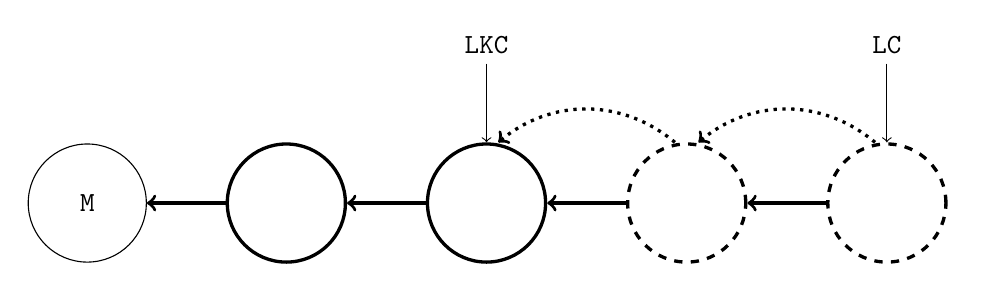
\begin{tikzpicture}[
			block/.style={circle, draw=black!100, very thick, minimum size=15mm},
			invis/.style={circle, draw=black!100, minimum size=15mm},
			label/.style={rectangle, text width=2cm, align=center}]                       
			\node[invis] (invis) {\texttt{M}};
			\node[block] (block1) [right=of invis] {};
			\node[block] (block2) [right=of block1] {};
			\node[label] (label1) [above=of block2] {\texttt{LKC}};
			\node[block] (block3) [right=of block2, dashed] {};
			\node[block] (block4) [right=of block3, dashed] {};
			\node[label] (label2) [above=of block4] {\texttt{LC}};
			\draw[->] (label2.south) -- (block4.north);
			\draw[->] (label1.south) -- (block2.north);
			\begin{scope}[very thick, -stealth]
				\draw[<-] (invis.east) -- (block1.west);
				\draw[<-] (block1.east) -- (block2.west);
				\draw[<-] (block2.east) -- (block3.west);
				\draw[<-] (block3.east) -- (block4.west);
				\path[dotted, ->] (block4.north)+(-1.5mm,0) edge  [bend right=40]  ([xshift=1.5mm]block3.north);
				\path[dotted, ->] (block3.north)+(-1.5mm,0) edge  [bend right=40]  ([xshift=1.5mm]block2.north);
			\end{scope}
		\end{tikzpicture}
		\caption{Retrieving Updates from a Single Participant Mempool}
		\label{fig:readmemudpates}
	\end{figure}
	Once the Leader has retrieved updates from the mempools of all Participants, it can order these transactions by their Ezirmin log item timestamp.
	After pulling updates from all Participants, the Leader can now see a list of newly retrieved transactions which are ordered by a timestamp.
	These updates can be validated and added to the blockchain, and the \textit{Latest Known Cursor} updated to the latest message in each of the mempool.\\

	However, this approach is fundamentally flawed and causes many updates to be seen out of order. 
	This is because of the delays that occur when mempool updates are retrieved over the network from multiple Participants.
	Figure \ref{fig:readremotepartudpatesbroke} demonstrates a typical situation where this occurs.
	The chains labelled \texttt{W} represent the mempools of Workers and the middle chain represents the stream of updates as seen by the Leader.\footnote{Here these udpates are shown as if they are part of a single merged mempool, although in reality they exist on isolated branches in the Leader's mempool, and are only merged by the Leader in memory.}
	In this figure, updates from the first worker will be pulled before updates from the second.
	However, after the first pull has taken place, the first Participant may have added additional transactions. 
	These transactions will be timestamped before the latest transaction in the second Participant's mempool, such that when the leader next polls for updates, transactions will be found which have a timestamp before the latest item committed to the blockchain.
	These items should have been committed first as they have an earlier timestamp.
	This transaction cannot be inserted into an earlier position of the blockchain because it would mean that different Participants might observe the blockchain in diverging states.
	It is not clear whether or not these transactions should be committed late or skipped, but ideally all transactions should be committed to the blockchain in the order that they were committed at Participants.
	I shall refer to these transactions as \textit{missed}.\\

	\begin{figure}
		\centering
		\begin{subfigure}[t]{0.45\textwidth}
			\centering
			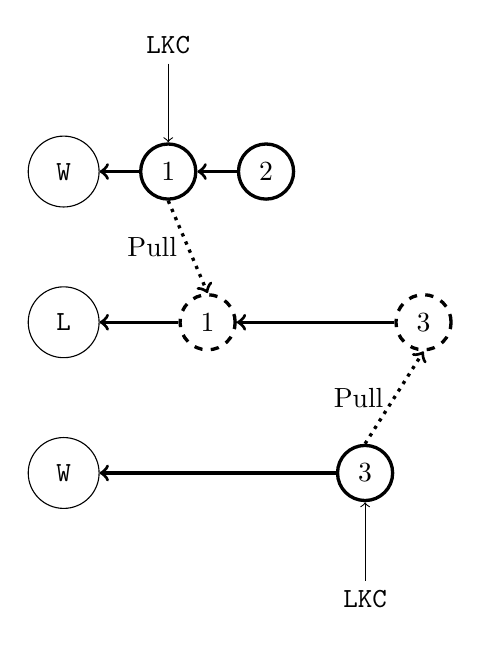
\begin{tikzpicture}[
				block/.style={circle, draw=black!100, very thick, minimum size=7mm},
				invis/.style={circle, draw=black!100, minimum size=9mm},
				label/.style={rectangle, text width=1.2cm, align=center}
			]
			\node[invis] (gentop) {\texttt{W}};
			\node[invis] (genmiddle) [below=of gentop] {\texttt{L}};
			\node[invis] (genbottom) [below=of genmiddle] {\texttt{W}};
			\node[block] (one) [right=5mm of gentop] {1};
			\node[block] (onemerged) [right=10mm of genmiddle, dashed] {1};
			\node[block] (two) [right=5mm of one] {2};
			\node[block] (three) [right=30mm of genbottom] {3};
			\node[block] (threemerged) [right=20mm of onemerged, dashed] {3};
			\node[label] (latestknownone) [above=of one] {\texttt{LKC}};
			\node[label] (latestknownthree) [below=of three] {\texttt{LKC}};
			\draw[->] (latestknownone.south) -- (one.north);
			\draw[->] (latestknownthree.north) -- (three.south);
			\begin{scope}[very thick, -stealth]
			\draw[<-] (gentop.east) -- (one.west);
			\draw[dotted, ->] (one.south) -- (onemerged.north) node[midway, left] {Pull};
			\draw[dotted, ->] (three.north) -- (threemerged.south) node[midway, left] {Pull};
			\draw[<-] (onemerged.east) -- (threemerged.west);
			\draw[<-] (one.east) -- (two.west);
			\draw[<-] (genmiddle.east) -- (onemerged.west);
			\draw[<-] (genbottom.east) -- (three.west);
			\end{scope}
			\end{tikzpicture}
		\caption{After first Leader poll. Transactions 1 and 3 are recognised by the Leader and added to the blockchain.}
		\end{subfigure}
		\begin{subfigure}[t]{0.45\textwidth}
			\centering
			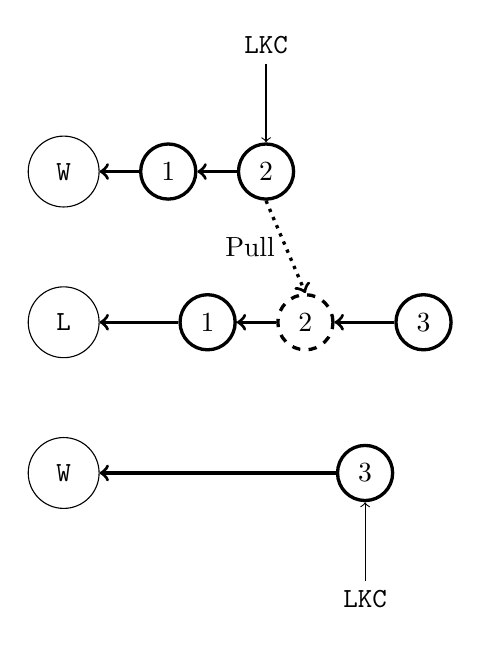
\begin{tikzpicture}[
				block/.style={circle, draw=black!100, very thick, minimum size=7mm},
				invis/.style={circle, draw=black!100, minimum size=9mm},
				label/.style={rectangle, text width=1.2cm, align=center}
			]
			\node[invis] (gentop) {\texttt{W}};
			\node[invis] (genmiddle) [below=of gentop] {\texttt{L}};
			\node[invis] (genbottom) [below=of genmiddle] {\texttt{W}};
			\node[block] (one) [right=5mm of gentop] {1};
			\node[block] (onemerged) [right=10mm of genmiddle] {1};
			\node[block] (two) [right=5mm of one] {2};
			\node[block] (twomerged) [right=5mm of onemerged, dashed] {2};
			\node[block] (three) [right=30mm of genbottom] {3};
			\node[block] (threemerged) [right=20mm of onemerged] {3};
			\node[label] (latestknowntwo) [above=of two] {\texttt{LKC}};
			\node[label] (latestknownthree) [below=of three] {\texttt{LKC}};
			\draw[->] (latestknowntwo.south) -- (two.north);
			\draw[->] (latestknownthree.north) -- (three.south);
			\begin{scope}[very thick, -stealth]
			\draw[<-] (gentop.east) -- (one.west);
			\draw[dotted, ->] (two.south) -- (twomerged.north) node[midway, left] {Pull};
			\draw[<-] (onemerged.east) -- (twomerged.west);
			\draw[<-] (twomerged.east) -- (threemerged.west);
			\draw[<-] (one.east) -- (two.west);
			\draw[<-] (genmiddle.east) -- (onemerged.west);
			\draw[<-] (genbottom.east) -- (three.west);
			\end{scope}
			\end{tikzpicture}
			\caption{After second Leader poll. Transaction 2 is retrieved but should be ordered before transaction 3 in the blockchain.}
		\end{subfigure}
		\caption{Missing mempool updates with a na\"{i}ve consensus mechanism}	
		\label{fig:readremotepartudpatesbroke}
	\end{figure}

	In order to solve this problem, I first examined the nature of these \textit{missed} transactions and noted the following properties:
	\begin{enumerate}
		\item Missed transactions must have been added whilst the Leader is pulling updates. 
		If they occurred before the poll had begun, then they would have been retrieved in previous poll. 
		Alternatively, missed transactions must occur after the latest timestamped transaction from the previous pull. 
		\item Missed transactions must have been added at a point in time earlier than the latest update from a round of retrieved updates.
		If they occurred at a later point in time, then they would be correctly received by the subsequent Leader poll.
	\end{enumerate}

	\subsubsection*{A Complex Approach}
	These properties naturally suggest a less na{\"i}ve algorithm for retrieving updates which only adds updates that have existed for more than one `poll cycle'.
	Once the Leader has retrieved a set of updates, it will add them to a \textit{retrieved} buffer.
	In the next poll cycle, the Leader will transfer the retrieved buffer to a new \textit{to-be-committed} buffer.
	The Leader now retrieves new updates from mempools, as before, and will do one of two things for each newly retrieved transaction:
	\begin{itemize}
		\item If a transaction is earlier that the latest transaction in the to-be-committed buffer, the Leader will insert it into the position in the buffer based on its timestamp.
		\item If a transaction is later than the latest transaction in the to-be-committed buffer, the Leader will add it to the retrieved buffer.
	\end{itemize}
	Figure \ref{fig:complexconsensusfix} demonstrates how this approach would solve the problem presented in Figure \ref{fig:readremotepartudpatesbroke}.
	In a), transaction 2 has been missed whilst transactions 1 and 3 have been added to the retrieved buffer. 
	In b), transactions 1, 2 and 3 have been inserted into the to-be-committed buffer and will be added to the blockchain.
	Transaction 4 has occurred after the latest item in the to-be-committed buffer, i.e. transaction 3, and is therefore added to the retrieved buffer instead. \\

	\begin{figure}
		\centering
		\begin{subfigure}[t]{\textwidth}
			\centering
			\begin{tikzpicture}[
				block/.style={circle, draw=black!100, very thick, minimum size=7mm},
				invis/.style={circle, draw=black!100, minimum size=9mm},
				label/.style={rectangle, text width=1.2cm, align=center},
				buffer/.style={rectangle, align=center},
				bufferitem/.style={rectangle, draw=black!100, align=center},
				spacer/.style={rectangle, text=white}
			]
			\node[invis] (gentop) {\texttt{W}};
			\node[invis] (genmiddle) [below=of gentop] {\texttt{L}};
			\node[invis] (genbottom) [below=of genmiddle] {\texttt{W}};
			\node[block] (one) [right=5mm of gentop] {1};
			\node[block] (onemerged) [right=10mm of genmiddle, dashed] {1};
			\node[block] (two) [right=5mm of one] {2};
			\node[block] (three) [right=30mm of genbottom] {3};
			\node[block] (threemerged) [right=20mm of onemerged, dashed] {3};
			\node[label] (latestknownone) [above=of one] {\texttt{LKC}};
			\node[label] (latestknownthree) [below=of three] {\texttt{LKC}};
			\draw[->] (latestknownone.south) -- (one.north);
			\draw[->] (latestknownthree.north) -- (three.south);
			\node[buffer] (bufferlabel) [right=2cm of threemerged] {Retrieved Buffer:};
			\node[bufferitem] (item1) [right=1cm of bufferlabel] {1};
			\node[bufferitem] (item2) [right=0mm of item1] {3};
			\node[spacer] (space1) [below=5mm of item1] {.};
			\begin{scope}[very thick, -stealth]
			\draw[<-] (gentop.east) -- (one.west);
			\draw[dotted, ->] (one.south) -- (onemerged.north) node[midway, left] {Pull};
			\draw[dotted, ->] (three.north) -- (threemerged.south) node[midway, left] {Pull};
			\draw[<-] (onemerged.east) -- (threemerged.west);
			\draw[<-] (one.east) -- (two.west);
			\draw[<-] (genmiddle.east) -- (onemerged.west);
			\draw[<-] (genbottom.east) -- (three.west);
			\end{scope}
			\end{tikzpicture}
		\caption{After first poll.}
		\end{subfigure}
		\begin{subfigure}[t]{\textwidth}
			\centering
			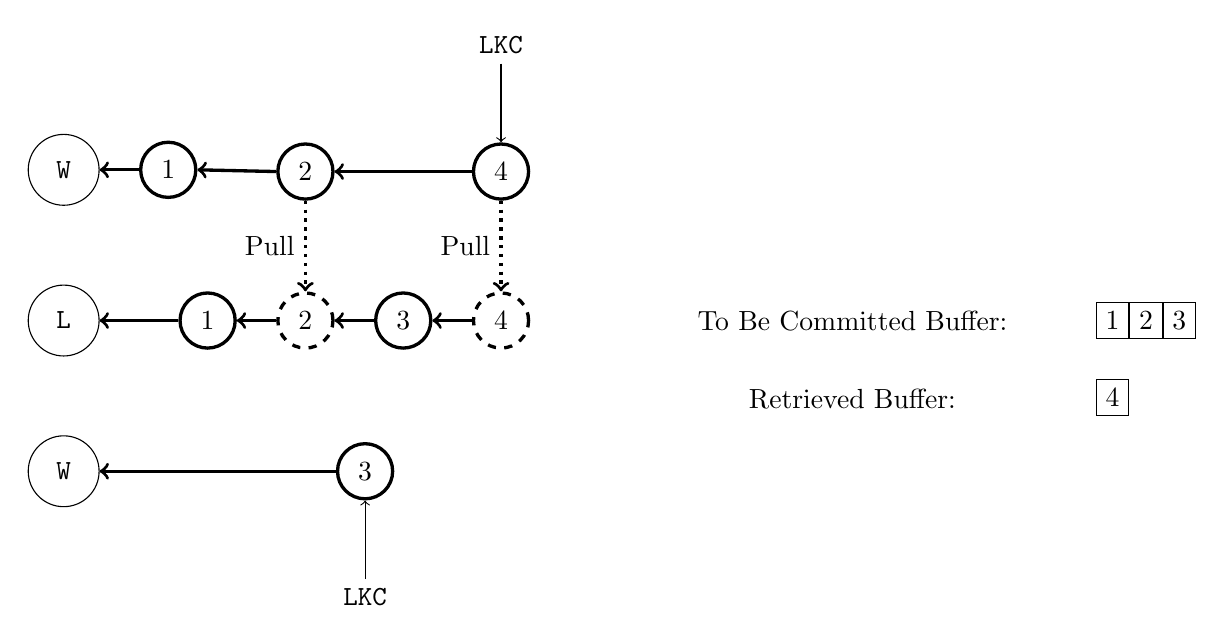
\begin{tikzpicture}[
				block/.style={circle, draw=black!100, very thick, minimum size=7mm},
				invis/.style={circle, draw=black!100, minimum size=9mm},
				label/.style={rectangle, text width=1.2cm, align=center},
				buffer/.style={rectangle},
				bufferitem/.style={rectangle, draw=black!100, align=center},
				spacer/.style={rectangle, text=white}
			]
			\node[invis] (gentop) {\texttt{W}};
			\node[spacer] (space) [above=1cm of gentop] {.};
			\node[invis] (genmiddle) [below=of gentop] {\texttt{L}};
			\node[invis] (genbottom) [below=of genmiddle] {\texttt{W}};
			\node[block] (one) [right=5mm of gentop] {1};
			\node[block] (onemerged) [right=10mm of genmiddle] {1};
			\node[block] (twomerged) [right=5mm of onemerged, dashed] {2};
			\node[block] (two) [above=1.15cm of twomerged] {2};
			\node[block] (three) [right=30mm of genbottom] {3};
			\node[block] (threemerged) [right=5mm of twomerged] {3};
			\node[block] (fourmerged) [right=5mm of threemerged, dashed] {4};
			\node[block] (four) [above=1.15cm of fourmerged] {4};
			\node[buffer] (txnslabel) [right=2cm of fourmerged] {To Be Committed Buffer:};
			\node[bufferitem] (item1) [right=1cm of txnslabel] {1};
			\node[bufferitem] (item2) [right=0mm of item1] {2};
			\node[bufferitem] (item3) [right=0mm of item2] {3};
			\node[label] (latestknownfour) [above=of four] {\texttt{LKC}};
			\node[label] (latestknownthree) [below=of three] {\texttt{LKC}};
			\draw[->] (latestknownfour.south) -- (four.north);
			\draw[->] (latestknownthree.north) -- (three.south);
			\node[buffer] (bufferlabel) [below=5mm of txnslabel] {Retrieved Buffer:};
			\node[bufferitem] (item1) [below=5mm of item1] {4};
			\node[spacer] (space1) [below=5mm of item1] {.};
			\begin{scope}[very thick, -stealth]
			\draw[<-] (gentop.east) -- (one.west);
			\draw[dotted, ->] (two.south) -- (twomerged.north) node[midway, left] {Pull};
			\draw[dotted, ->] (four.south) -- (fourmerged.north) node[midway, left] {Pull};
			\draw[<-] (onemerged.east) -- (twomerged.west);
			\draw[<-] (twomerged.east) -- (threemerged.west);
			\draw[<-] (one.east) -- (two.west);
			\draw[<-] (two.east) -- (four.west);
			\draw[<-] (genmiddle.east) -- (onemerged.west);
			\draw[<-] (genbottom.east) -- (three.west);
			\draw[<-] (threemerged.east) -- (fourmerged.west);
			\end{scope}
			\end{tikzpicture}
			\caption{After second Leader poll.}
		\end{subfigure}
		\caption{Buffering Updates in a Complex Consensus Mechanism}	
		\label{fig:complexconsensusfix}
	\end{figure}

	Now I have detailed all the work that I have completed to build Logan.
	Transactions are sourced from the mempool and added to the blockchain when it can be certain that there will be no missed transactions.
	Transactions are added in order and never changed such that if a Participant observes the state of the blockchain at any point, it will never observe a conflicting state in the future.
	The algorithm used by Logan assumes that clock timestamps are synchronised across all devices.
	This may not be the case in an arbitrary situation, and consequently, in high load situations some transactions may not be recognised in the correct order. 
	However, the system is not built for systems of such high load and I do not consider this to be a large issue. 

	\chapter{Evaluation}
	%introduction to evaluation and metrics used

	\subsection*{Metrics Used}
	In order to evaluate the performance of Logan, I have looked at two key metrics: latency and throughput.
	In a blockchain system, it is important that the latency is as low as possible. 
	Latency dictates how long a user must wait before they can be sure that their transaction has been added.
	It is easy to see why this is important by thinking in terms of a cryptocurrency application.
	In this context long latencies will cause users to become irritated and potentially stop using your currency.
	Throughput is also a useful measure because it shows how well a system can cope with large loads.
	Again in the context of a cryptocurrency, it is important that lots of users should be able to make transactions at the same time.
	As with all distributed systems, these two metrics are inevitably linked, and higher system throughputs will lead to larger latencies. 
	In the worst case, a large throughput will cause the system to become overloaded, latencies will rise and throughput will even descrease!
	I have looked at how the throughput applied to the system affects the latency of Logan transactions, in order to try to determine the optimal use case conditions for a Logan system.\\

	I have also looked at how the latency of adding transactions varies with the size of the blockchain at a constant throughput.
	It is important that the system should be able to work well even when the size of the blockchain is large so that performance will not degrade over time.
	
	\section{Performance on a Local Machine}
	%TODO detail how performance varies on a single machine 
	\subsection{Single Participant}
	%What happens when there is one participant only?
	Figure \ref{fig:singlocal} shows how the latency of transactions varies with throughput for a Participant node on the same machine as the Leader node.
	Latency stays at between 10-15ms up until the system reaches about 70 transactions per second.
	The set of data points which lie significantly above the straight line are points where the system has become overloaded. 
	The rate of transactions has become so high that latencies have increased and the throughput has actually decreased again. 
	This is a really interesting result because it shows that Logan's logic functions well at throughputs of between 50 and 60 transactions per second, whilst maintaining low transaction latency.
	These figures are much better than my success criteria which suggested the system should be able to cope with around 2-3 transactions per second.\\
	\begin{figure}
		\centering
		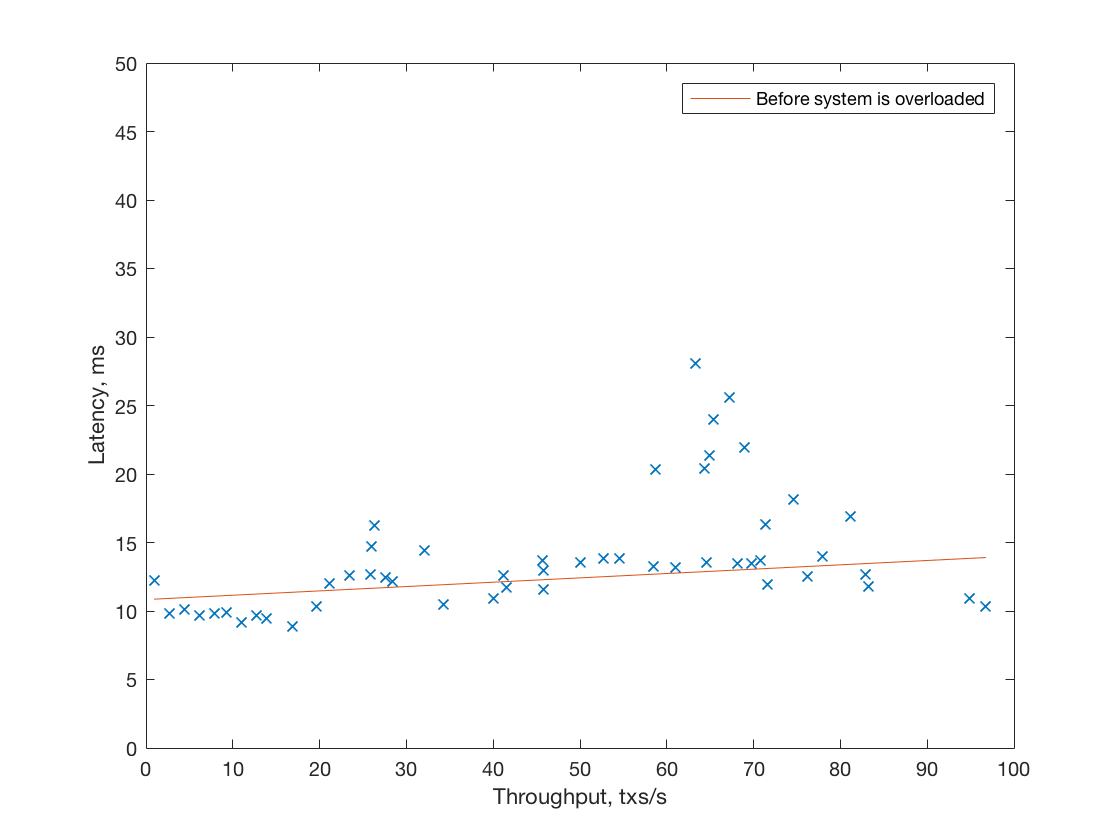
\includegraphics[width=0.8\textwidth]{figs/single_local_worker.png}
		\caption{Latency variation with throughput on a single local Participant}
		\label{fig:singlocal}
	\end{figure}

	Figure \ref{fig:locallatency} shows how the latency of Logan transactions varies as the size of the blockchain increases. 
	The Figure shows clearly that the latency of adding a transaction is constant in the size of the blockchain.
	This is a very desirable trait as it means that Logan can be used for systems that run for indefinite periods of time, with arbitrary long blockchain histories.
	In the requirements analysis, I set out the criteria that Logan should be able to add transactions at constant latency and this result shows that I have been successful in achieving this criteria.\\
	\begin{figure}
		\centering
		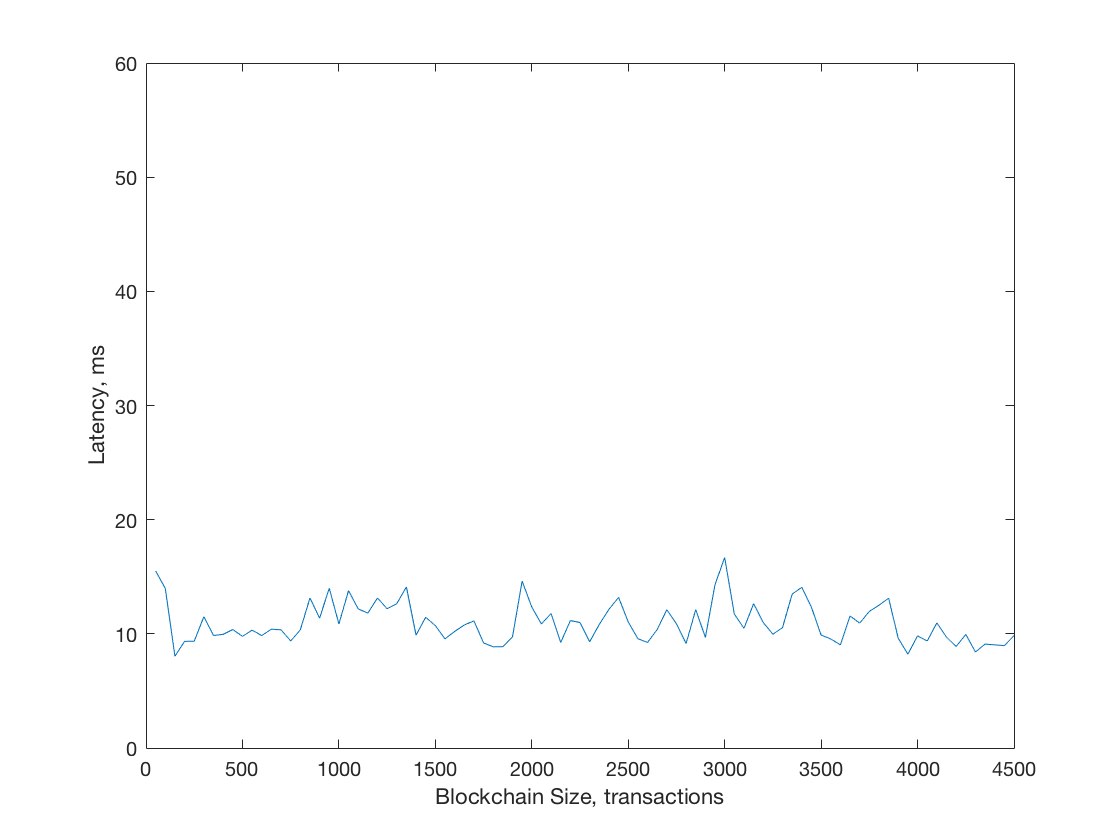
\includegraphics[width=0.8\textwidth]{figs/latency_vs_size.png}
		\caption{Latency variation with blockchain size on a local Participant}
		\label{fig:locallatency}
	\end{figure}

	The graph also compares latencies when a simple, constant-time validator is used, which blindly accepts all transactions, and when no validation is performed. 
	The result without validation was obtained by removing the validation code completely from the codebase and just accepting all transactions.
	Intuitively, these two results should be the same because they perform the same logical task, and this graph confirms this intuition. 
	From this, we can conclude that if a user provides a constant time algorithm for validating transactions, then the overall time for adding transactions will remain constant.
	
	\subsection{Multiple Participants}
	%What about with multiple particpants

	\section{Performance on Remote Machines}
	%How does performance vary when there are multiple machines
	\subsection{Single Remote Participant}
	In order to see how the system performs when network latencies are involved, I first looked at Logan's performance when there is just one Leader and one remote Participant.
	Figure \ref{figs:remlatencysize} shows how the latency of adding a Logan transaction changes as ths size of the blockchain increases, with a fixed throughput.
	\begin{figure}
		\centering
		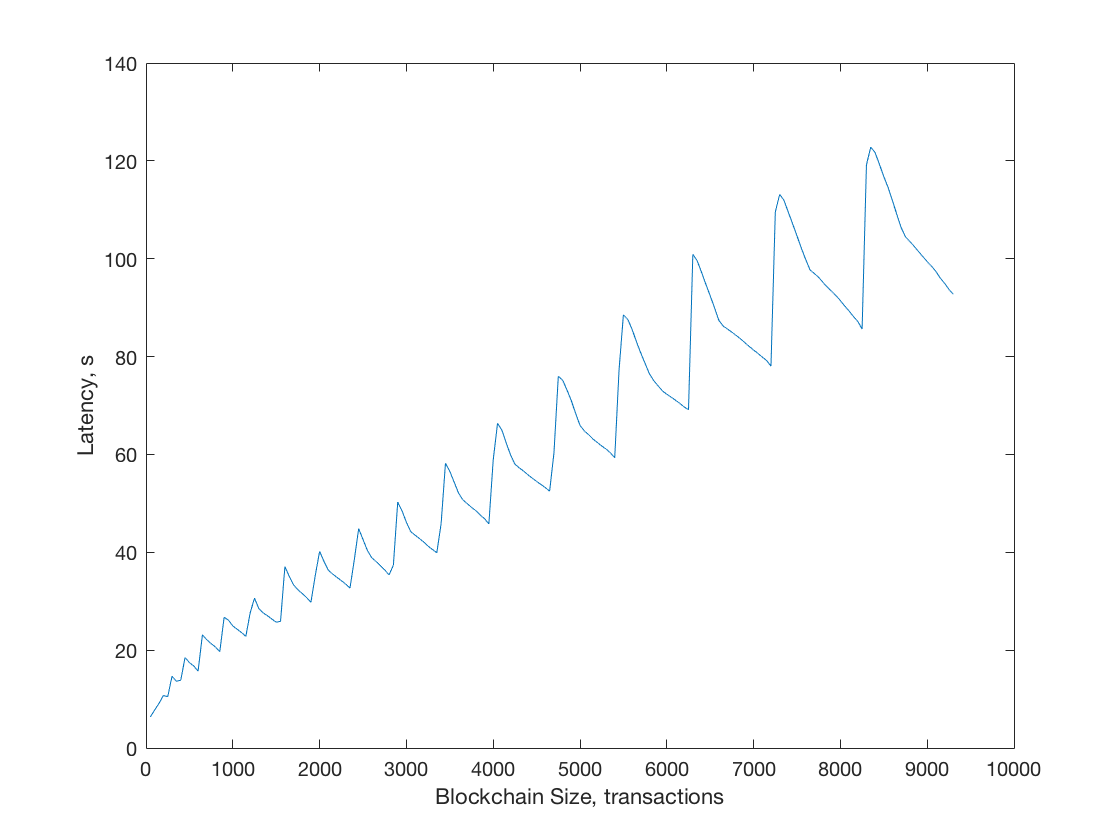
\includegraphics[width=0.8\textwidth]{figs/remote_latency_size.png}
		\caption{Logan latencies with increasing blockchain size}
		\label{figs:remlatencysize}
	\end{figure}
	The two interesting features of this graph are the saw-tooth shape, and the linear increase in latency.
	The saw-tooth shape is due to the nature of the Leader polls.
	When a Leader pulls new updates into its mempool, some of these updates will be older than others, and will therefore experience a higher latency than the most recently added updates. 
	The troughs in the graph represent the transactions which were added immediately before the Leader pulled in new updates.
	The peaks, on the other hand, represent the transactions added immediately after the Leader pulled in new updates.
	These transactions will have waited for that entire poll cycle to complete, before being seen by the Leader.\\

	The second interesting feature of the graph is the linear increase in latency. 
	In order to see what was causing this, I logged the time that the Leader spends completing all of its computational tasks for every poll cycle, and plotted how these delays increase with the blockchain size.
	Figure \ref{figs:leaderdelays} compares the delays in Leader polls with the number of updates that is pulled in each poll cycle.
	\begin{figure}
		\centering
		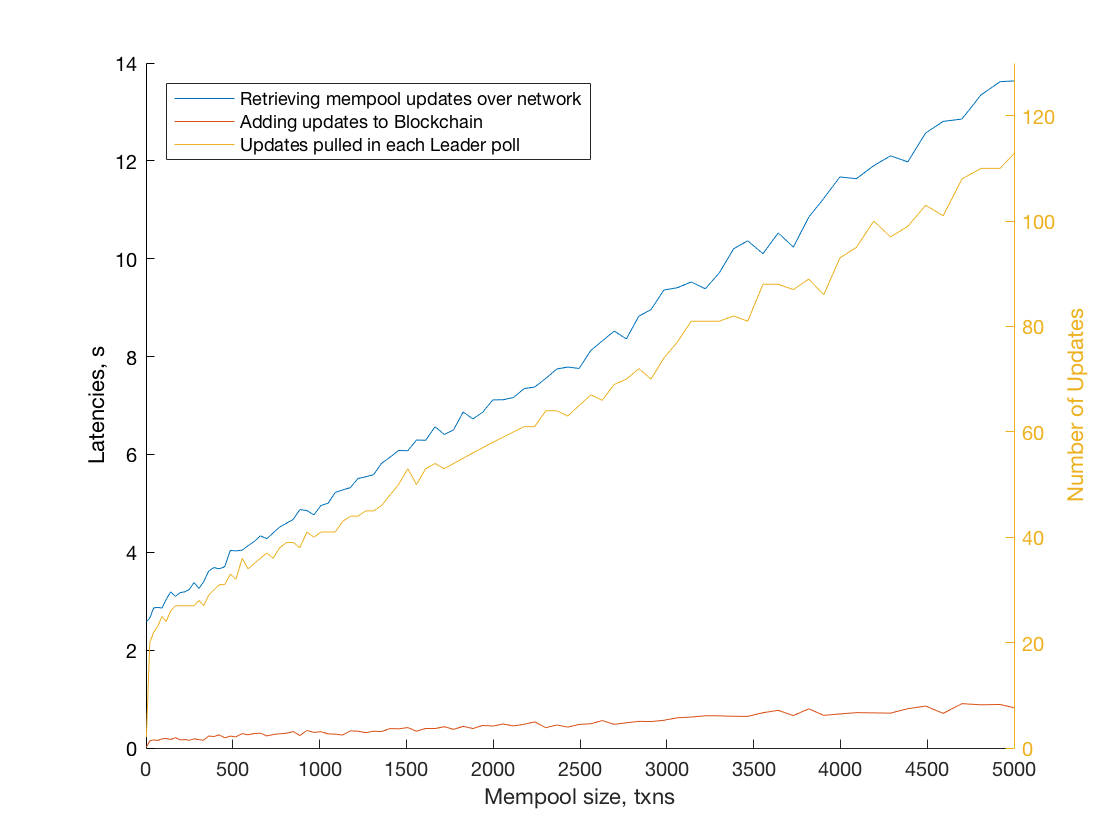
\includegraphics[width=0.8\textwidth]{figs/leader_delays_num_pulled.png}
		\caption{Delays incurred by Leader for every poll cycle}
		\label{figs:leaderdelays}
	\end{figure}
	There is a clear correlation between the number of updates pulled and the latency in both adding them to the blockchain, and pulling them over the network, but it is not immediately clear what the causation here is.
	The increase in the time taken adding updates to the blockchain can be put down to the increased number of updates being added. 
	Intuitively this is a linear time operation that will grow as the number of updates found in a poll cycle increases.
	Additionally, Figure \ref{fig:locallatency} shows that when the number of updates in a poll is constant, so is the time taken adding them to the blockchain.
	This means that the increasing delay of adding updates to the blockhain can be assigned to the delay that is causing the overall latency, or number of updates found, to rise.
	Therefore, to find the underlying cause of this is, I examined the overheads of pulling updates over a network with Git alone and with Ezirmin's \texttt{Sync} module.\\

	Figure \ref{figs:gitoverheads} compares the latencies of the \texttt{git pull} command with the latencies of using the \texttt{Sync.pull} command provided by Ezirmin.
	\begin{figure}
		\centering
		\begin{subfigure}[t]{\textwidth}
			\centering
			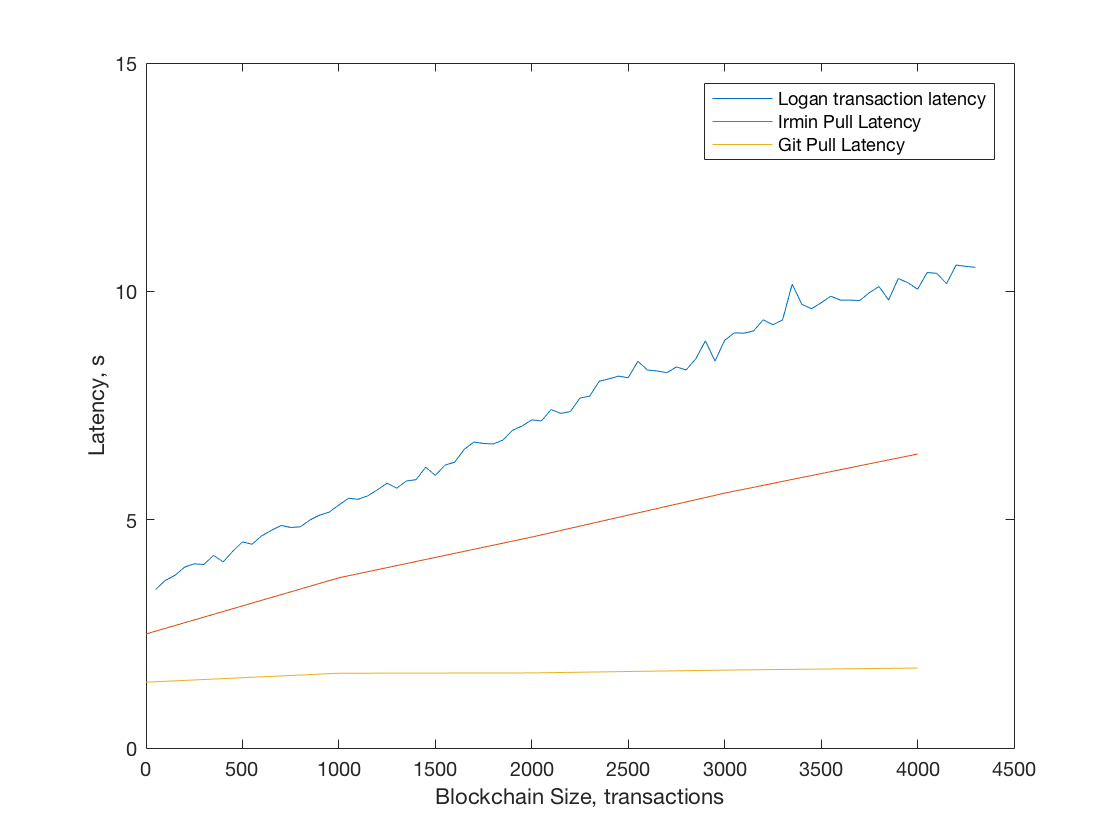
\includegraphics[width=0.9\textwidth]{figs/gitlatencies.png}
			\caption{Latencies of pulling 100 transactions against blockchain size}
			\label{figs:gitreposize}
		\end{subfigure}
		
		\begin{subfigure}[t]{\textwidth}
			\centering
			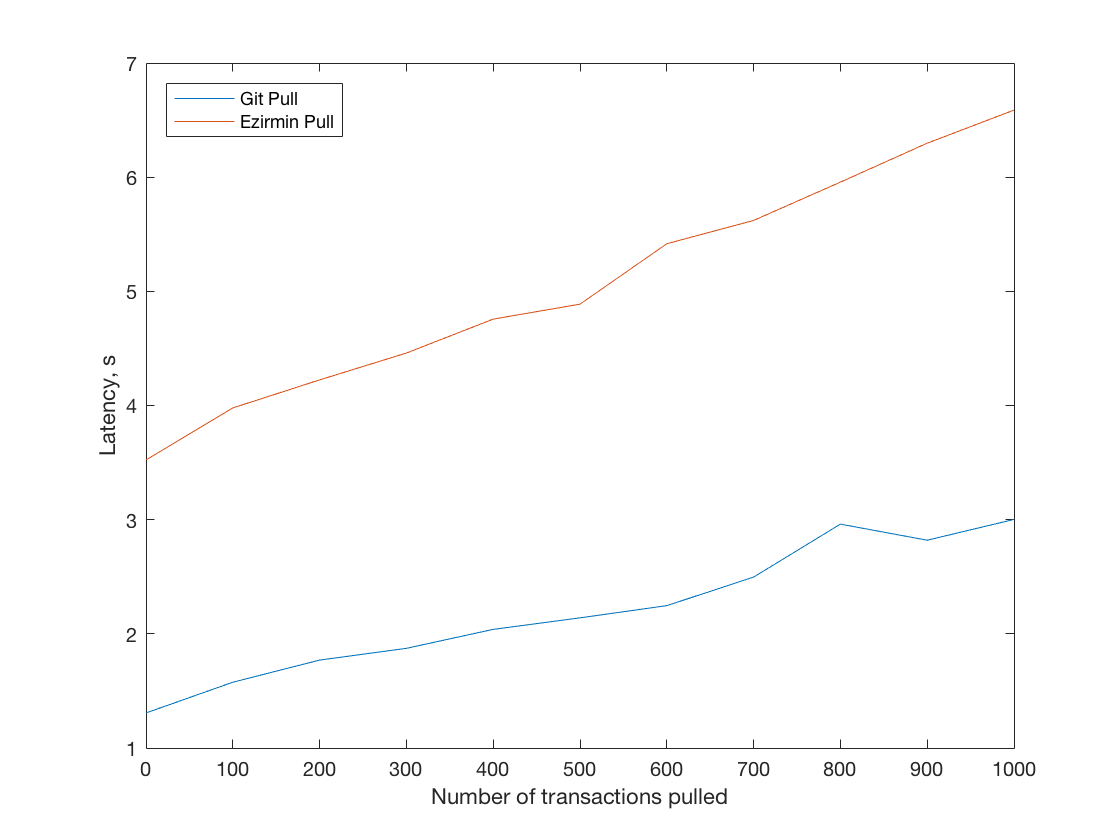
\includegraphics[width=0.9\textwidth]{figs/gitlatenciespullsize.png}
			\caption{Latencies of pulling increasing number of transactions}
			\label{figs:gitpullsize}
		\end{subfigure}
		\caption{Git and Ezirmin Sync overheads}
		\label{figs:gitoverheads}
	\end{figure}
	Figure \ref{figs:gitreposize} shows that whilst the latency of \texttt{git pull} is pretty much constant, the latency of using Ezirmin to pull updates increases linearly as the size of the mempool increases

	Figure \ref{figs:gitpullsize} shows that the latency of using Git increases linearly with the number of transactions pulled.
	This is an intuitive result that is unfortunately unavoidable due to network delays, data compression etc.
	More importantly however, this graph shows that not only is the Ezirmin implementation of this functionality much slower, but it also grows at a faster rate.

	\subsection{Multiple Remote Participants}

	\chapter{Conclusion}
	
	
	%%%%%%%%%%%%%%%%%%%%%%%%%%%%%%%%%%%%%%%%%%%%%%%%%%%%%%%%%%%%%%%%%%%%%
	% the bibliography
	\bibliographystyle{acm}
	\bibliography{refs}
	\addcontentsline{toc}{chapter}{Bibliography}
	
	%%%%%%%%%%%%%%%%%%%%%%%%%%%%%%%%%%%%%%%%%%%%%%%%%%%%%%%%%%%%%%%%%%%%%
	% the appendices
	\appendix

	\chapter{Project Proposal}
	
	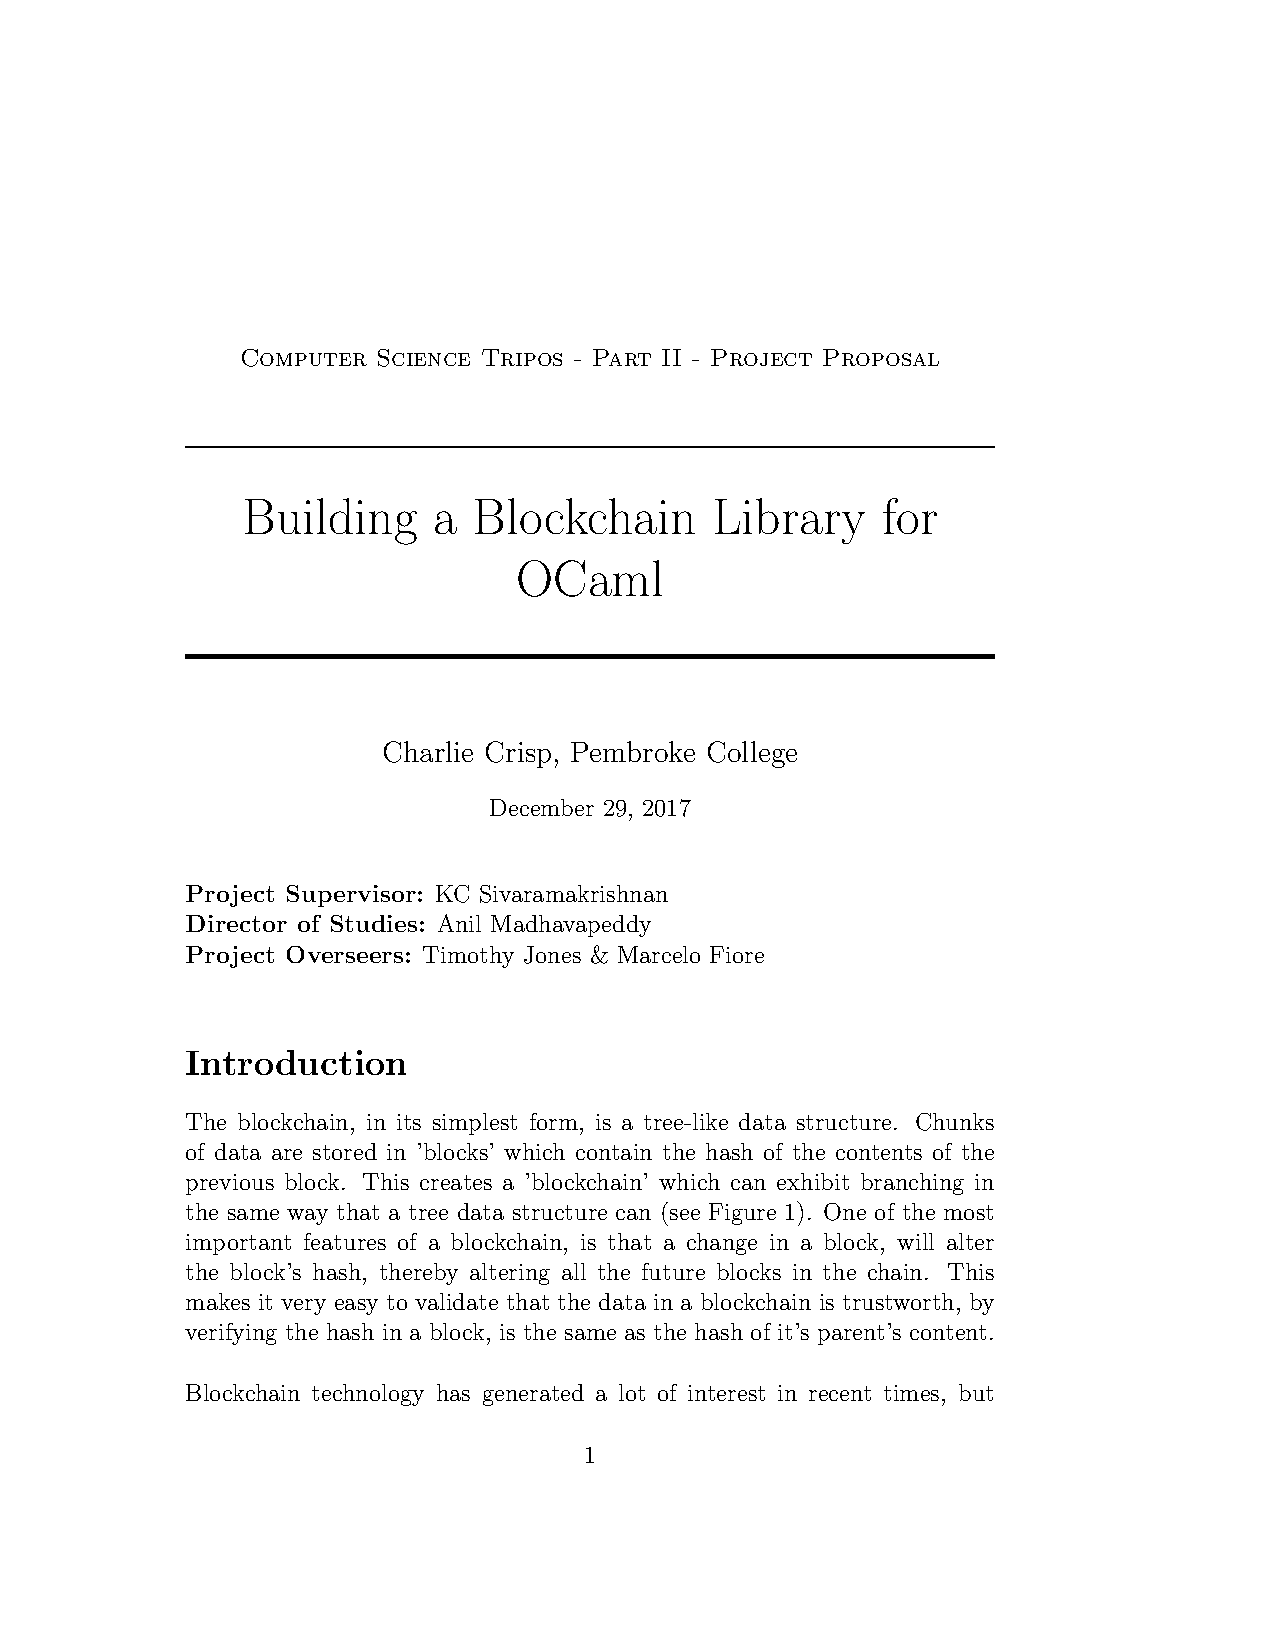
\includepdf[pages=-]{Part_II_Project_Proposal_Draft.pdf}
	
	\end{document}